\documentclass[pdflatex,sn-basic]{sn-jnl}

\usepackage[T1]{fontenc}
\usepackage{lmodern}
\usepackage{graphicx}
\usepackage{amsmath,amssymb,amsfonts}
\usepackage{amsthm}
\usepackage{booktabs}
\usepackage{array}
\newcolumntype{P}[1]{>{\raggedright\arraybackslash}p{#1}}
\usepackage{multirow}
\usepackage{xcolor}
\usepackage{algorithm}
\usepackage{algorithmicx}
\usepackage{algpseudocode}
\usepackage{pifont}
\usepackage{xr-hyper}
\usepackage{hyperref}
\externaldocument[S-]{supplement}

\graphicspath{{../../code/figures/}}
% Generated by code/experiments/aggregate.py -- do not edit by hand.
\newcommand{\AUROCAblFaultsFiniteC}{0.729}
\newcommand{\AUROCAblFaultsFreeB}{0.653}
\newcommand{\AUROCAblFaultsHoldoutPairs}{0.754}
\newcommand{\AUROCAblFaultsInSample}{0.770}
\newcommand{\AUROCAblFaultsKNN}{0.725}
\newcommand{\AUROCAblFaultsLambdaSSE}{0.775}
\newcommand{\AUROCAblFaultsLoom}{0.765}
\newcommand{\AUROCAblFaultsNoSmooth}{0.747}
\newcommand{\AUROCAblFaultsPreVal}{0.563}
\newcommand{\AUROCAblFaultsPreValSmooth}{0.553}
\newcommand{\AUROCFaultsHoldoutTS}{0.558}
\newcommand{\AUROCFaultsIsotonic}{0.592}
\newcommand{\AUROCFaultsLogReg}{0.516}
\newcommand{\AUROCFaultsLoom}{0.765}
\newcommand{\AUROCFaultsOnehot}{0.500}
\newcommand{\AUROCFaultsPlatt}{0.610}
\newcommand{\AUROCFaultsPreVal}{0.563}
\newcommand{\AUROCFaultsQuant}{0.709}
\newcommand{\AUROCFaultsSoftmax}{0.531}
\newcommand{\AUROCOffSevThreeArsenal}{0.676}
\newcommand{\AUROCOffSevThreeLoom}{0.845}
\newcommand{\AUROCOffSevThreeLoomEns}{0.847}
\newcommand{\AUROCOffSevThreePreVal}{0.531}
\newcommand{\AUROCOffSevThreePreValEns}{0.584}
\newcommand{\AUROCOffSevThreeQuant}{0.760}
\newcommand{\AccCleanHoldoutTS}{0.896}
\newcommand{\AccCleanIsotonic}{0.904}
\newcommand{\AccCleanLogReg}{0.901}
\newcommand{\AccCleanLoom}{0.914}
\newcommand{\AccCleanOnehot}{0.914}
\newcommand{\AccCleanPlatt}{0.912}
\newcommand{\AccCleanPreVal}{0.914}
\newcommand{\AccCleanQuant}{0.895}
\newcommand{\AccCleanSoftmax}{0.914}
\newcommand{\AccFaultsHoldoutTS}{0.676}
\newcommand{\AccFaultsIsotonic}{0.682}
\newcommand{\AccFaultsLogReg}{0.660}
\newcommand{\AccFaultsLoom}{0.695}
\newcommand{\AccFaultsOnehot}{0.696}
\newcommand{\AccFaultsPlatt}{0.697}
\newcommand{\AccFaultsPreVal}{0.692}
\newcommand{\AccFaultsQuant}{0.694}
\newcommand{\AccFaultsSoftmax}{0.696}
\newcommand{\AccOffCleanArsenal}{0.900}
\newcommand{\AccOffCleanLoom}{0.905}
\newcommand{\AccOffCleanLoomEns}{0.907}
\newcommand{\AccOffCleanPreVal}{0.910}
\newcommand{\AccOffCleanPreValEns}{0.910}
\newcommand{\AccOffCleanQuant}{0.883}
\newcommand{\AccOffSevThreeArsenal}{0.600}
\newcommand{\AccOffSevThreeLoom}{0.604}
\newcommand{\AccOffSevThreeLoomEns}{0.614}
\newcommand{\AccOffSevThreePreVal}{0.613}
\newcommand{\AccOffSevThreePreValEns}{0.616}
\newcommand{\AccOffSevThreeQuant}{0.621}
\newcommand{\BayesAUROCPreValBetter}{1.00}
\newcommand{\BayesAUROCPreValEquiv}{0.00}
\newcommand{\BayesAUROCPreValWorse}{0.00}
\newcommand{\BayesCleanPreValBetter}{0.38}
\newcommand{\BayesCleanPreValEquiv}{0.00}
\newcommand{\BayesCleanPreValWorse}{0.62}
\newcommand{\BayesConfirmCaughtPreValBetter}{1.00}
\newcommand{\BayesConfirmCaughtPreValEquiv}{0.00}
\newcommand{\BayesConfirmCaughtPreValWorse}{0.00}
\newcommand{\BayesConfirmCaughtQuantBetter}{1.00}
\newcommand{\BayesConfirmCaughtQuantEquiv}{0.00}
\newcommand{\BayesConfirmCaughtQuantWorse}{0.00}
\newcommand{\BayesConfirmErrPreValBetter}{0.98}
\newcommand{\BayesConfirmErrPreValEquiv}{0.02}
\newcommand{\BayesConfirmErrPreValWorse}{0.00}
\newcommand{\BayesConfirmErrQuantBetter}{0.30}
\newcommand{\BayesConfirmErrQuantEquiv}{0.14}
\newcommand{\BayesConfirmErrQuantWorse}{0.56}
\newcommand{\BayesFaultsPreValBetter}{1.00}
\newcommand{\BayesFaultsPreValEquiv}{0.00}
\newcommand{\BayesFaultsPreValWorse}{0.00}
\newcommand{\BayesFaultsQuantBetter}{0.14}
\newcommand{\BayesFaultsQuantEquiv}{0.00}
\newcommand{\BayesFaultsQuantWorse}{0.86}
\newcommand{\BayesQFQuantBetter}{0.00}
\newcommand{\BayesQFQuantEquiv}{0.00}
\newcommand{\BayesQFQuantWorse}{1.00}
\newcommand{\BayesRealNoisePreValBetter}{1.00}
\newcommand{\BayesRealNoisePreValEquiv}{0.00}
\newcommand{\BayesRealNoisePreValWorse}{0.00}
\newcommand{\BrierCleanHoldoutTS}{0.177}
\newcommand{\BrierCleanIsotonic}{0.157}
\newcommand{\BrierCleanLogReg}{0.151}
\newcommand{\BrierCleanLoom}{0.144}
\newcommand{\BrierCleanOnehot}{0.171}
\newcommand{\BrierCleanPlatt}{0.148}
\newcommand{\BrierCleanPreVal}{0.134}
\newcommand{\BrierCleanQuant}{0.210}
\newcommand{\BrierCleanSoftmax}{0.284}
\newcommand{\BrierFaultsHoldoutTS}{0.532}
\newcommand{\BrierFaultsIsotonic}{0.491}
\newcommand{\BrierFaultsLogReg}{0.527}
\newcommand{\BrierFaultsLoom}{0.435}
\newcommand{\BrierFaultsOnehot}{0.608}
\newcommand{\BrierFaultsPlatt}{0.462}
\newcommand{\BrierFaultsPreVal}{0.510}
\newcommand{\BrierFaultsQuant}{0.415}
\newcommand{\BrierFaultsSoftmax}{0.537}
\newcommand{\BrierOffCleanArsenal}{0.173}
\newcommand{\BrierOffCleanLoom}{0.163}
\newcommand{\BrierOffCleanLoomEns}{0.165}
\newcommand{\BrierOffCleanPreVal}{0.140}
\newcommand{\BrierOffCleanPreValEns}{0.137}
\newcommand{\BrierOffCleanQuant}{0.219}
\newcommand{\BrierOffSevThreeArsenal}{0.672}
\newcommand{\BrierOffSevThreeLoom}{0.526}
\newcommand{\BrierOffSevThreeLoomEns}{0.519}
\newcommand{\BrierOffSevThreePreVal}{0.673}
\newcommand{\BrierOffSevThreePreValEns}{0.636}
\newcommand{\BrierOffSevThreeQuant}{0.489}
\newcommand{\CCaughtHoldoutTS}{23\,\%}
\newcommand{\CCaughtLoom}{41\,\%}
\newcommand{\CCaughtPlatt}{28\,\%}
\newcommand{\CCaughtPreVal}{24\,\%}
\newcommand{\CCaughtQuant}{34\,\%}
\newcommand{\CErrCleanHoldoutTS}{9.8\,\%}
\newcommand{\CErrCleanLoom}{4.4\,\%}
\newcommand{\CErrCleanPlatt}{4.6\,\%}
\newcommand{\CErrCleanPreVal}{4.8\,\%}
\newcommand{\CErrCleanQuant}{8.9\,\%}
\newcommand{\CErrHoldoutTS}{19.8\,\%}
\newcommand{\CErrLoom}{10.1\,\%}
\newcommand{\CErrPlatt}{15.0\,\%}
\newcommand{\CErrPreVal}{14.6\,\%}
\newcommand{\CErrQuant}{13.2\,\%}
\newcommand{\CIAUROCFaultsDiffHoldoutTS}{-0.228 [-0.252, -0.202]}
\newcommand{\CIAUROCFaultsDiffPlatt}{-0.160 [-0.186, -0.136]}
\newcommand{\CIAUROCFaultsDiffPreVal}{-0.226 [-0.252, -0.200]}
\newcommand{\CIAUROCFaultsDiffQuant}{-0.052 [-0.065, -0.040]}
\newcommand{\CIAUROCFaultsHoldoutTS}{0.543 [0.523, 0.562]}
\newcommand{\CIAUROCFaultsLoom}{0.770 [0.751, 0.788]}
\newcommand{\CIAUROCFaultsPlatt}{0.610 [0.584, 0.634]}
\newcommand{\CIAUROCFaultsPreVal}{0.544 [0.524, 0.564]}
\newcommand{\CIAUROCFaultsQuant}{0.718 [0.700, 0.735]}
\newcommand{\CICCaughtLoom}{43.4\,\% [39.4, 47.5]}
\newcommand{\CICCaughtPreVal}{26.0\,\% [23.2, 29.2]}
\newcommand{\CICCaughtQuant}{34.8\,\% [31.4, 38.4]}
\newcommand{\CICErrLoom}{15.6\,\% [10.8, 20.5]}
\newcommand{\CICErrPreVal}{17.3\,\% [12.6, 22.2]}
\newcommand{\CICErrQuant}{16.8\,\% [12.2, 22.0]}
\newcommand{\CIECECleanDiffHoldoutTS}{-0.021 [-0.029, -0.013]}
\newcommand{\CIECECleanDiffPlatt}{0.018 [0.009, 0.031]}
\newcommand{\CIECECleanDiffPreVal}{-0.031 [-0.039, -0.023]}
\newcommand{\CIECECleanDiffQuant}{0.046 [0.031, 0.061]}
\newcommand{\CIECECleanHoldoutTS}{0.065 [0.051, 0.084]}
\newcommand{\CIECECleanLoom}{0.086 [0.072, 0.106]}
\newcommand{\CIECECleanPlatt}{0.096 [0.081, 0.114]}
\newcommand{\CIECECleanPreVal}{0.055 [0.042, 0.075]}
\newcommand{\CIECECleanQuant}{0.132 [0.116, 0.150]}
\newcommand{\CINLLCleanDiffHoldoutTS}{0.235 [0.146, 0.336]}
\newcommand{\CINLLCleanDiffPlatt}{0.041 [0.000, 0.099]}
\newcommand{\CINLLCleanDiffPreVal}{0.026 [-0.005, 0.065]}
\newcommand{\CINLLCleanDiffQuant}{0.075 [0.025, 0.131]}
\newcommand{\CINLLCleanHoldoutTS}{0.664 [0.550, 0.796]}
\newcommand{\CINLLCleanLoom}{0.429 [0.356, 0.511]}
\newcommand{\CINLLCleanPlatt}{0.425 [0.357, 0.509]}
\newcommand{\CINLLCleanPreVal}{0.456 [0.375, 0.541]}
\newcommand{\CINLLCleanQuant}{0.504 [0.426, 0.602]}
\newcommand{\CINLLFaultsDiffHoldoutTS}{2.516 [1.973, 3.057]}
\newcommand{\CINLLFaultsDiffPlatt}{0.632 [0.437, 0.828]}
\newcommand{\CINLLFaultsDiffPreVal}{1.996 [1.489, 2.501]}
\newcommand{\CINLLFaultsDiffQuant}{0.084 [-0.014, 0.186]}
\newcommand{\CINLLFaultsHoldoutTS}{3.452 [2.882, 4.016]}
\newcommand{\CINLLFaultsLoom}{0.936 [0.825, 1.051]}
\newcommand{\CINLLFaultsPlatt}{1.525 [1.284, 1.773]}
\newcommand{\CINLLFaultsPreVal}{2.932 [2.406, 3.480]}
\newcommand{\CINLLFaultsQuant}{1.020 [0.870, 1.191]}
\newcommand{\CIRNLoom}{1.438 [1.150, 1.761]}
\newcommand{\CIRNPreVal}{6.137 [4.436, 7.955]}
\newcommand{\CNDatasets}{38}
\newcommand{\CPLoomAPSCovClean}{90.8\,\%}
\newcommand{\CPLoomAPSCovFaults}{90.5\,\%}
\newcommand{\CPLoomAPSEmptyClean}{7.3\,\%}
\newcommand{\CPLoomAPSEmptyFaults}{1.5\,\%}
\newcommand{\CPLoomAPSSizeClean}{5.22}
\newcommand{\CPLoomAPSSizeFaults}{6.62}
\newcommand{\CPLoomCovAlphaFive}{95.1\,\%}
\newcommand{\CPLoomCovAlphaTwenty}{79.6\,\%}
\newcommand{\CPLoomCovClean}{89.8\,\%}
\newcommand{\CPLoomCovFaults}{63.8\,\%}
\newcommand{\CPLoomEmptyClean}{4.6\,\%}
\newcommand{\CPLoomEmptyFaults}{25.0\,\%}
\newcommand{\CPLoomSizeClean}{1.55}
\newcommand{\CPLoomSizeFaults}{1.66}
\newcommand{\CPPreValCovClean}{90.8\,\%}
\newcommand{\CPPreValCovFaults}{69.6\,\%}
\newcommand{\CPPreValEmptyClean}{3.3\,\%}
\newcommand{\CPPreValEmptyFaults}{9.3\,\%}
\newcommand{\CPPreValSizeClean}{1.58}
\newcommand{\CPPreValSizeFaults}{1.55}
\newcommand{\CPSplitCovClean}{92.8\,\%}
\newcommand{\CPSplitCovFaults}{76.3\,\%}
\newcommand{\CPSplitEmptyClean}{2.2\,\%}
\newcommand{\CPSplitEmptyFaults}{6.8\,\%}
\newcommand{\CPSplitSizeClean}{2.49}
\newcommand{\CPSplitSizeFaults}{2.38}
\newcommand{\CmpAUROCAblFaultsFiniteC}{better on 111 of 114 datasets, $p<0.001$}
\newcommand{\CmpAUROCAblFaultsFreeB}{better on 112 of 114 datasets, $p<0.001$}
\newcommand{\CmpAUROCAblFaultsHoldoutPairs}{better on 85 of 114 datasets, $p<0.001$}
\newcommand{\CmpAUROCAblFaultsInSample}{not significantly different, with 49 wins and 62 losses of 114 datasets, $p=0.650$}
\newcommand{\CmpAUROCAblFaultsKNN}{better on 107 of 114 datasets, $p<0.001$}
\newcommand{\CmpAUROCAblFaultsLambdaSSE}{worse on 63 of 114 datasets, $p=0.004$}
\newcommand{\CmpAUROCAblFaultsNoSmooth}{better on 87 of 114 datasets, $p<0.001$}
\newcommand{\CmpAUROCAblFaultsPreVal}{better on 114 of 114 datasets, $p<0.001$}
\newcommand{\CmpAUROCAblFaultsPreValSmooth}{better on 114 of 114 datasets, $p<0.001$}
\newcommand{\CmpAUROCFaultsHoldoutTS}{better on 114 of 114 datasets, $p<0.001$}
\newcommand{\CmpAUROCFaultsIsotonic}{better on 105 of 110 datasets, $p<0.001$}
\newcommand{\CmpAUROCFaultsLogReg}{better on 109 of 109 datasets, $p<0.001$}
\newcommand{\CmpAUROCFaultsOnehot}{better on 114 of 114 datasets, $p<0.001$}
\newcommand{\CmpAUROCFaultsPlatt}{better on 101 of 110 datasets, $p<0.001$}
\newcommand{\CmpAUROCFaultsPreVal}{better on 114 of 114 datasets, $p<0.001$}
\newcommand{\CmpAUROCFaultsQuant}{better on 97 of 114 datasets, $p<0.001$}
\newcommand{\CmpAUROCFaultsSoftmax}{better on 114 of 114 datasets, $p<0.001$}
\newcommand{\CmpAUROCOffSevThreeArsenal}{better on 109 of 113 datasets, $p<0.001$}
\newcommand{\CmpAUROCOffSevThreeLoomEns}{worse on 82 of 114 datasets, $p<0.001$}
\newcommand{\CmpAUROCOffSevThreePreVal}{better on 114 of 114 datasets, $p<0.001$}
\newcommand{\CmpAUROCOffSevThreePreValEns}{better on 114 of 114 datasets, $p<0.001$}
\newcommand{\CmpAUROCOffSevThreeQuant}{better on 99 of 114 datasets, $p<0.001$}
\newcommand{\CmpAccCleanHoldoutTS}{better on 91 of 114 datasets, $p<0.001$}
\newcommand{\CmpAccCleanIsotonic}{better on 73 of 110 datasets, $p<0.001$}
\newcommand{\CmpAccCleanLogReg}{better on 78 of 109 datasets, $p<0.001$}
\newcommand{\CmpAccCleanOnehot}{not significantly different, with 28 wins and 42 losses of 114 datasets, $p=0.572$}
\newcommand{\CmpAccCleanPlatt}{not significantly different, with 41 wins and 50 losses of 110 datasets, $p=0.849$}
\newcommand{\CmpAccCleanPreVal}{not significantly different, with 28 wins and 29 losses of 114 datasets, $p=0.572$}
\newcommand{\CmpAccCleanQuant}{not significantly different, with 63 wins and 47 losses of 114 datasets, $p=0.572$}
\newcommand{\CmpAccCleanSoftmax}{not significantly different, with 28 wins and 42 losses of 114 datasets, $p=0.572$}
\newcommand{\CmpAccFaultsHoldoutTS}{better on 90 of 114 datasets, $p<0.001$}
\newcommand{\CmpAccFaultsIsotonic}{better on 82 of 110 datasets, $p<0.001$}
\newcommand{\CmpAccFaultsLogReg}{better on 89 of 109 datasets, $p<0.001$}
\newcommand{\CmpAccFaultsOnehot}{not significantly different, with 37 wins and 47 losses of 114 datasets, $p=0.583$}
\newcommand{\CmpAccFaultsPlatt}{better on 74 of 110 datasets, $p=0.002$}
\newcommand{\CmpAccFaultsPreVal}{not significantly different, with 43 wins and 39 losses of 114 datasets, $p=0.729$}
\newcommand{\CmpAccFaultsQuant}{worse on 74 of 114 datasets, $p=0.011$}
\newcommand{\CmpAccFaultsSoftmax}{not significantly different, with 37 wins and 47 losses of 114 datasets, $p=0.583$}
\newcommand{\CmpAccOffCleanArsenal}{not significantly different, with 45 wins and 34 losses of 113 datasets, $p=0.967$}
\newcommand{\CmpAccOffCleanLoomEns}{worse on 44 of 114 datasets, $p=0.008$}
\newcommand{\CmpAccOffCleanPreVal}{not significantly different, with 10 wins and 10 losses of 114 datasets, $p=0.967$}
\newcommand{\CmpAccOffCleanPreValEns}{worse on 49 of 114 datasets, $p=0.008$}
\newcommand{\CmpAccOffCleanQuant}{not significantly different, with 52 wins and 43 losses of 114 datasets, $p=0.967$}
\newcommand{\CmpAccOffSevThreeArsenal}{not significantly different, with 57 wins and 54 losses of 113 datasets, $p=1.000$}
\newcommand{\CmpAccOffSevThreeLoomEns}{not significantly different, with 49 wins and 58 losses of 114 datasets, $p=1.000$}
\newcommand{\CmpAccOffSevThreePreVal}{not significantly different, with 19 wins and 19 losses of 114 datasets, $p=1.000$}
\newcommand{\CmpAccOffSevThreePreValEns}{not significantly different, with 46 wins and 64 losses of 114 datasets, $p=0.673$}
\newcommand{\CmpAccOffSevThreeQuant}{worse on 76 of 114 datasets, $p<0.001$}
\newcommand{\CmpBrierCleanHoldoutTS}{better on 75 of 114 datasets, $p<0.001$}
\newcommand{\CmpBrierCleanIsotonic}{not significantly different, with 55 wins and 55 losses of 110 datasets, $p=1.000$}
\newcommand{\CmpBrierCleanLogReg}{not significantly different, with 58 wins and 51 losses of 109 datasets, $p=0.528$}
\newcommand{\CmpBrierCleanOnehot}{better on 80 of 114 datasets, $p<0.001$}
\newcommand{\CmpBrierCleanPlatt}{not significantly different, with 46 wins and 64 losses of 110 datasets, $p=1.000$}
\newcommand{\CmpBrierCleanPreVal}{worse on 78 of 114 datasets, $p<0.001$}
\newcommand{\CmpBrierCleanQuant}{better on 71 of 114 datasets, $p=0.004$}
\newcommand{\CmpBrierCleanSoftmax}{better on 111 of 114 datasets, $p<0.001$}
\newcommand{\CmpBrierFaultsHoldoutTS}{better on 100 of 114 datasets, $p<0.001$}
\newcommand{\CmpBrierFaultsIsotonic}{better on 90 of 110 datasets, $p<0.001$}
\newcommand{\CmpBrierFaultsLogReg}{better on 99 of 109 datasets, $p<0.001$}
\newcommand{\CmpBrierFaultsOnehot}{better on 106 of 114 datasets, $p<0.001$}
\newcommand{\CmpBrierFaultsPlatt}{better on 77 of 110 datasets, $p<0.001$}
\newcommand{\CmpBrierFaultsPreVal}{better on 93 of 114 datasets, $p<0.001$}
\newcommand{\CmpBrierFaultsQuant}{worse on 76 of 114 datasets, $p=0.008$}
\newcommand{\CmpBrierFaultsSoftmax}{better on 102 of 114 datasets, $p<0.001$}
\newcommand{\CmpBrierOffCleanArsenal}{better on 69 of 113 datasets, $p<0.001$}
\newcommand{\CmpBrierOffCleanLoomEns}{worse on 76 of 114 datasets, $p<0.001$}
\newcommand{\CmpBrierOffCleanPreVal}{worse on 81 of 114 datasets, $p<0.001$}
\newcommand{\CmpBrierOffCleanPreValEns}{worse on 90 of 114 datasets, $p<0.001$}
\newcommand{\CmpBrierOffCleanQuant}{better on 68 of 114 datasets, $p=0.006$}
\newcommand{\CmpBrierOffSevThreeArsenal}{better on 96 of 113 datasets, $p<0.001$}
\newcommand{\CmpBrierOffSevThreeLoomEns}{worse on 75 of 114 datasets, $p<0.001$}
\newcommand{\CmpBrierOffSevThreePreVal}{better on 99 of 114 datasets, $p<0.001$}
\newcommand{\CmpBrierOffSevThreePreValEns}{better on 93 of 114 datasets, $p<0.001$}
\newcommand{\CmpBrierOffSevThreeQuant}{worse on 83 of 114 datasets, $p<0.001$}
\newcommand{\CmpCCaughtGrouped}{better on 27 of 27 source-level units, $p<0.001$}
\newcommand{\CmpCCaughtHoldoutTS}{better on 38 of 38 datasets, $p<0.001$}
\newcommand{\CmpCCaughtPlatt}{better on 33 of 37 datasets, $p<0.001$}
\newcommand{\CmpCCaughtPreVal}{better on 38 of 38 datasets, $p<0.001$}
\newcommand{\CmpCCaughtQuant}{better on 34 of 38 datasets, $p<0.001$}
\newcommand{\CmpCErrHoldoutTS}{better on 37 of 38 datasets, $p<0.001$}
\newcommand{\CmpCErrPlatt}{better on 31 of 37 datasets, $p<0.001$}
\newcommand{\CmpCErrPreVal}{better on 35 of 38 datasets, $p<0.001$}
\newcommand{\CmpCErrQuant}{not significantly different, with 17 wins and 20 losses of 38 datasets, $p=0.635$}
\newcommand{\CmpECEAblCleanFiniteC}{worse on 88 of 114 datasets, $p<0.001$}
\newcommand{\CmpECEAblCleanFreeB}{worse on 86 of 114 datasets, $p<0.001$}
\newcommand{\CmpECEAblCleanHoldoutPairs}{better on 101 of 114 datasets, $p<0.001$}
\newcommand{\CmpECEAblCleanInSample}{better on 110 of 114 datasets, $p<0.001$}
\newcommand{\CmpECEAblCleanKNN}{not significantly different, with 51 wins and 63 losses of 114 datasets, $p=0.186$}
\newcommand{\CmpECEAblCleanLambdaSSE}{worse on 33 of 114 datasets, $p=0.003$}
\newcommand{\CmpECEAblCleanNoSmooth}{worse on 84 of 114 datasets, $p<0.001$}
\newcommand{\CmpECEAblCleanPreVal}{worse on 86 of 114 datasets, $p<0.001$}
\newcommand{\CmpECEAblCleanPreValSmooth}{worse on 78 of 114 datasets, $p<0.001$}
\newcommand{\CmpECEAblFaultsFiniteC}{worse on 77 of 114 datasets, $p=0.002$}
\newcommand{\CmpECEAblFaultsFreeB}{not significantly different, with 62 wins and 52 losses of 114 datasets, $p=0.614$}
\newcommand{\CmpECEAblFaultsHoldoutPairs}{better on 87 of 114 datasets, $p<0.001$}
\newcommand{\CmpECEAblFaultsInSample}{better on 99 of 114 datasets, $p<0.001$}
\newcommand{\CmpECEAblFaultsKNN}{not significantly different, with 46 wins and 68 losses of 114 datasets, $p=0.213$}
\newcommand{\CmpECEAblFaultsLambdaSSE}{not significantly different, with 52 wins and 36 losses of 114 datasets, $p=0.213$}
\newcommand{\CmpECEAblFaultsNoSmooth}{worse on 75 of 114 datasets, $p<0.001$}
\newcommand{\CmpECEAblFaultsPreVal}{better on 80 of 114 datasets, $p<0.001$}
\newcommand{\CmpECEAblFaultsPreValSmooth}{better on 76 of 114 datasets, $p=0.001$}
\newcommand{\CmpECECleanHoldoutTS}{worse on 72 of 114 datasets, $p<0.001$}
\newcommand{\CmpECECleanIsotonic}{worse on 80 of 110 datasets, $p<0.001$}
\newcommand{\CmpECECleanLogReg}{worse on 73 of 109 datasets, $p<0.001$}
\newcommand{\CmpECECleanOnehot}{better on 62 of 114 datasets, $p=0.005$}
\newcommand{\CmpECECleanPlatt}{better on 71 of 110 datasets, $p<0.001$}
\newcommand{\CmpECECleanPreVal}{worse on 86 of 114 datasets, $p<0.001$}
\newcommand{\CmpECECleanQuant}{better on 85 of 114 datasets, $p<0.001$}
\newcommand{\CmpECECleanSoftmax}{better on 108 of 114 datasets, $p<0.001$}
\newcommand{\CmpECEFaultsHoldoutTS}{better on 86 of 114 datasets, $p<0.001$}
\newcommand{\CmpECEFaultsIsotonic}{not significantly different, with 56 wins and 54 losses of 110 datasets, $p=1.000$}
\newcommand{\CmpECEFaultsLogReg}{better on 78 of 109 datasets, $p<0.001$}
\newcommand{\CmpECEFaultsOnehot}{better on 93 of 114 datasets, $p<0.001$}
\newcommand{\CmpECEFaultsPlatt}{not significantly different, with 55 wins and 55 losses of 110 datasets, $p=1.000$}
\newcommand{\CmpECEFaultsPreVal}{better on 80 of 114 datasets, $p<0.001$}
\newcommand{\CmpECEFaultsQuant}{better on 75 of 114 datasets, $p=0.005$}
\newcommand{\CmpECEFaultsSoftmax}{better on 105 of 114 datasets, $p<0.001$}
\newcommand{\CmpGroupedFaults}{better on 68 of 70 source-level units, $p<0.001$}
\newcommand{\CmpHydraClean}{not significantly different, with 43 wins and 67 losses of 110 datasets, $p=0.147$}
\newcommand{\CmpHydraFaults}{better on 106 of 110 datasets, $p<0.001$}
\newcommand{\CmpMRClean}{worse on 72 of 110 datasets, $p=0.008$}
\newcommand{\CmpMRFaults}{better on 105 of 110 datasets, $p<0.001$}
\newcommand{\CmpNLLAblCleanFiniteC}{worse on 89 of 114 datasets, $p<0.001$}
\newcommand{\CmpNLLAblCleanFreeB}{worse on 84 of 114 datasets, $p<0.001$}
\newcommand{\CmpNLLAblCleanHoldoutPairs}{better on 110 of 113 datasets, $p<0.001$}
\newcommand{\CmpNLLAblCleanInSample}{better on 113 of 114 datasets, $p<0.001$}
\newcommand{\CmpNLLAblCleanKNN}{not significantly different, with 58 wins and 56 losses of 114 datasets, $p=1.000$}
\newcommand{\CmpNLLAblCleanLambdaSSE}{not significantly different, with 49 wins and 39 losses of 114 datasets, $p=0.079$}
\newcommand{\CmpNLLAblCleanNoSmooth}{not significantly different, with 53 wins and 60 losses of 114 datasets, $p=0.541$}
\newcommand{\CmpNLLAblCleanPreVal}{not significantly different, with 49 wins and 65 losses of 114 datasets, $p=1.000$}
\newcommand{\CmpNLLAblCleanPreValSmooth}{worse on 75 of 114 datasets, $p=0.038$}
\newcommand{\CmpNLLAblFaultsFiniteC}{not significantly different, with 50 wins and 64 losses of 114 datasets, $p=1.000$}
\newcommand{\CmpNLLAblFaultsFreeB}{better on 80 of 114 datasets, $p<0.001$}
\newcommand{\CmpNLLAblFaultsHoldoutPairs}{better on 94 of 113 datasets, $p<0.001$}
\newcommand{\CmpNLLAblFaultsInSample}{better on 108 of 114 datasets, $p<0.001$}
\newcommand{\CmpNLLAblFaultsKNN}{not significantly different, with 52 wins and 62 losses of 114 datasets, $p=1.000$}
\newcommand{\CmpNLLAblFaultsLambdaSSE}{not significantly different, with 42 wins and 46 losses of 114 datasets, $p=1.000$}
\newcommand{\CmpNLLAblFaultsNoSmooth}{better on 71 of 114 datasets, $p=0.003$}
\newcommand{\CmpNLLAblFaultsPreVal}{better on 108 of 114 datasets, $p<0.001$}
\newcommand{\CmpNLLAblFaultsPreValSmooth}{better on 94 of 114 datasets, $p<0.001$}
\newcommand{\CmpNLLCleanHoldoutTS}{better on 85 of 114 datasets, $p<0.001$}
\newcommand{\CmpNLLCleanIsotonic}{better on 96 of 110 datasets, $p<0.001$}
\newcommand{\CmpNLLCleanLogReg}{not significantly different, with 53 wins and 56 losses of 109 datasets, $p=1.000$}
\newcommand{\CmpNLLCleanOnehot}{better on 103 of 114 datasets, $p<0.001$}
\newcommand{\CmpNLLCleanPlatt}{not significantly different, with 53 wins and 57 losses of 110 datasets, $p=1.000$}
\newcommand{\CmpNLLCleanPreVal}{not significantly different, with 49 wins and 65 losses of 114 datasets, $p=1.000$}
\newcommand{\CmpNLLCleanQuant}{better on 77 of 114 datasets, $p<0.001$}
\newcommand{\CmpNLLCleanSoftmax}{better on 110 of 114 datasets, $p<0.001$}
\newcommand{\CmpNLLFaultsHoldoutTS}{better on 110 of 114 datasets, $p<0.001$}
\newcommand{\CmpNLLFaultsIsotonic}{better on 108 of 110 datasets, $p<0.001$}
\newcommand{\CmpNLLFaultsLogReg}{better on 104 of 109 datasets, $p<0.001$}
\newcommand{\CmpNLLFaultsOnehot}{better on 114 of 114 datasets, $p<0.001$}
\newcommand{\CmpNLLFaultsPlatt}{better on 86 of 110 datasets, $p<0.001$}
\newcommand{\CmpNLLFaultsPreVal}{better on 108 of 114 datasets, $p<0.001$}
\newcommand{\CmpNLLFaultsQuant}{not significantly different, with 44 wins and 70 losses of 114 datasets, $p=0.291$}
\newcommand{\CmpNLLFaultsSoftmax}{better on 105 of 114 datasets, $p<0.001$}
\newcommand{\CmpNLLOffCleanArsenal}{better on 94 of 113 datasets, $p<0.001$}
\newcommand{\CmpNLLOffCleanLoomEns}{worse on 76 of 114 datasets, $p<0.001$}
\newcommand{\CmpNLLOffCleanPreVal}{worse on 78 of 114 datasets, $p=0.003$}
\newcommand{\CmpNLLOffCleanPreValEns}{worse on 83 of 114 datasets, $p<0.001$}
\newcommand{\CmpNLLOffCleanQuant}{better on 70 of 114 datasets, $p=0.004$}
\newcommand{\CmpNLLOffSevThreeArsenal}{better on 110 of 113 datasets, $p<0.001$}
\newcommand{\CmpNLLOffSevThreeLoomEns}{worse on 76 of 114 datasets, $p<0.001$}
\newcommand{\CmpNLLOffSevThreePreVal}{better on 105 of 114 datasets, $p<0.001$}
\newcommand{\CmpNLLOffSevThreePreValEns}{better on 104 of 114 datasets, $p<0.001$}
\newcommand{\CmpNLLOffSevThreeQuant}{worse on 78 of 114 datasets, $p=0.042$}
\newcommand{\CmpNoDupClean}{not significantly different, with 42 wins and 56 losses of 98 datasets, $p=1.000$}
\newcommand{\CmpNoDupFaults}{better on 92 of 98 datasets, $p<0.001$}
\newcommand{\CmpNoNearDupClean}{not significantly different, with 39 wins and 51 losses of 90 datasets, $p=1.000$}
\newcommand{\CmpNoNearDupFaults}{better on 84 of 90 datasets, $p<0.001$}
\newcommand{\CmpQFAUROCQuant}{better on 93 of 110 datasets, $p<0.001$}
\newcommand{\CmpQFPreVal}{better on 110 of 110 datasets, $p<0.001$}
\newcommand{\CmpQFQuant}{worse on 97 of 110 datasets, $p<0.001$}
\newcommand{\CmpRNAUROCCellsPlatt}{better on 55 of 63 dataset--noise combinations, $p<0.001$}
\newcommand{\CmpRNAUROCCellsPreVal}{better on 63 of 63 dataset--noise combinations, $p<0.001$}
\newcommand{\CmpRNAUROCCellsQuant}{better on 54 of 63 dataset--noise combinations, $p<0.001$}
\newcommand{\CmpRNCellsPlatt}{better on 39 of 63 dataset--noise combinations, $p<0.001$}
\newcommand{\CmpRNCellsPreVal}{better on 50 of 63 dataset--noise combinations, $p<0.001$}
\newcommand{\CmpRNCellsQuant}{not significantly different, with 28 wins and 35 losses of 63 dataset--noise combinations, $p=0.748$}
\newcommand{\CmpSetSizeSplit}{smaller on 103 of 114 datasets, $p<0.001$}
\newcommand{\CmpUnseenClean}{not significantly different, with 43 wins and 57 losses of 100 datasets, $p=1.000$}
\newcommand{\CmpUnseenFaults}{better on 94 of 100 datasets, $p<0.001$}
\newcommand{\CovOutside}{42\,\%}
\newcommand{\CovSDObs}{0.035}
\newcommand{\CovSDSim}{0.010}
\newcommand{\CovSDSimHi}{0.013}
\newcommand{\ECEAblCleanFiniteC}{0.070}
\newcommand{\ECEAblCleanFreeB}{0.066}
\newcommand{\ECEAblCleanHoldoutPairs}{0.136}
\newcommand{\ECEAblCleanInSample}{0.478}
\newcommand{\ECEAblCleanKNN}{0.075}
\newcommand{\ECEAblCleanLambdaSSE}{0.076}
\newcommand{\ECEAblCleanLoom}{0.075}
\newcommand{\ECEAblCleanNoSmooth}{0.041}
\newcommand{\ECEAblCleanPreVal}{0.040}
\newcommand{\ECEAblCleanPreValSmooth}{0.065}
\newcommand{\ECEAblFaultsFiniteC}{0.152}
\newcommand{\ECEAblFaultsFreeB}{0.148}
\newcommand{\ECEAblFaultsHoldoutPairs}{0.191}
\newcommand{\ECEAblFaultsInSample}{0.337}
\newcommand{\ECEAblFaultsKNN}{0.153}
\newcommand{\ECEAblFaultsLambdaSSE}{0.152}
\newcommand{\ECEAblFaultsLoom}{0.151}
\newcommand{\ECEAblFaultsNoSmooth}{0.139}
\newcommand{\ECEAblFaultsPreVal}{0.185}
\newcommand{\ECEAblFaultsPreValSmooth}{0.181}
\newcommand{\ECECleanHoldoutTS}{0.052}
\newcommand{\ECECleanIsotonic}{0.044}
\newcommand{\ECECleanLogReg}{0.049}
\newcommand{\ECECleanLoom}{0.075}
\newcommand{\ECECleanOnehot}{0.086}
\newcommand{\ECECleanPlatt}{0.080}
\newcommand{\ECECleanPreVal}{0.040}
\newcommand{\ECECleanQuant}{0.116}
\newcommand{\ECECleanSoftmax}{0.249}
\newcommand{\ECEFaultsHoldoutTS}{0.197}
\newcommand{\ECEFaultsIsotonic}{0.153}
\newcommand{\ECEFaultsLogReg}{0.219}
\newcommand{\ECEFaultsLoom}{0.151}
\newcommand{\ECEFaultsOnehot}{0.304}
\newcommand{\ECEFaultsPlatt}{0.144}
\newcommand{\ECEFaultsPreVal}{0.185}
\newcommand{\ECEFaultsQuant}{0.170}
\newcommand{\ECEFaultsSoftmax}{0.256}
\newcommand{\ExchKS}{0.12}
\newcommand{\ExchN}{110}
\newcommand{\ExchQNineLoo}{1.68}
\newcommand{\ExchQNineTest}{1.74}
\newcommand{\ExchReject}{19}
\newcommand{\FamLoomBetter}{noise, speed variation and misalignment}
\newcommand{\FamQuantBetter}{baseline wander, dropouts and spikes}
\newcommand{\FitArsenal}{4.47}
\newcommand{\FitEndToEndLoom}{0.31}
\newcommand{\FitLogReg}{3.67}
\newcommand{\FitLoom}{0.14}
\newcommand{\FitLoomEns}{2.25}
\newcommand{\FitPlatt}{0.26}
\newcommand{\FitPreVal}{0.14}
\newcommand{\FitQuant}{1.30}
\newcommand{\FitTransform}{0.17}
\newcommand{\HypFailed}{H1b}
\newcommand{\LRMaxDataset}{ShapesAll}
\newcommand{\LRMaxGain}{0.161}
\newcommand{\LRMedDefault}{0.2707}
\newcommand{\LRMedLong}{0.2711}
\newcommand{\LRN}{12}
\newcommand{\LevClean}{1.01}
\newcommand{\LevMissing}{8.6}
\newcommand{\LevNoise}{30.3}
\newcommand{\LevShift}{3.5}
\newcommand{\LevSpikes}{29.5}
\newcommand{\LevWander}{6.2}
\newcommand{\LevWarp}{1.26}
\newcommand{\NDatasets}{114}
\newcommand{\NDupExact}{16}
\newcommand{\NDupNear}{24}
\newcommand{\NDupNearOnly}{eight}
\newcommand{\NGrouped}{70}
\newcommand{\NHyp}{10}
\newcommand{\NHypPass}{nine}
\newcommand{\NLLAblCleanFiniteC}{0.287}
\newcommand{\NLLAblCleanFreeB}{0.280}
\newcommand{\NLLAblCleanHoldoutPairs}{0.441}
\newcommand{\NLLAblCleanInSample}{0.978}
\newcommand{\NLLAblCleanKNN}{0.292}
\newcommand{\NLLAblCleanLambdaSSE}{0.300}
\newcommand{\NLLAblCleanLoom}{0.295}
\newcommand{\NLLAblCleanNoSmooth}{0.348}
\newcommand{\NLLAblCleanPreVal}{0.360}
\newcommand{\NLLAblCleanPreValSmooth}{0.290}
\newcommand{\NLLAblFaultsFiniteC}{0.775}
\newcommand{\NLLAblFaultsFreeB}{0.964}
\newcommand{\NLLAblFaultsHoldoutPairs}{0.846}
\newcommand{\NLLAblFaultsInSample}{1.096}
\newcommand{\NLLAblFaultsKNN}{0.771}
\newcommand{\NLLAblFaultsLambdaSSE}{0.751}
\newcommand{\NLLAblFaultsLoom}{0.738}
\newcommand{\NLLAblFaultsNoSmooth}{1.049}
\newcommand{\NLLAblFaultsPreVal}{1.728}
\newcommand{\NLLAblFaultsPreValSmooth}{1.172}
\newcommand{\NLLCleanHoldoutTS}{0.524}
\newcommand{\NLLCleanIsotonic}{0.670}
\newcommand{\NLLCleanLogReg}{0.314}
\newcommand{\NLLCleanLoom}{0.295}
\newcommand{\NLLCleanOnehot}{2.959}
\newcommand{\NLLCleanPlatt}{0.294}
\newcommand{\NLLCleanPreVal}{0.360}
\newcommand{\NLLCleanQuant}{0.386}
\newcommand{\NLLCleanSoftmax}{0.588}
\newcommand{\NLLFaultsHoldoutTS}{2.221}
\newcommand{\NLLFaultsIsotonic}{4.358}
\newcommand{\NLLFaultsLogReg}{1.878}
\newcommand{\NLLFaultsLoom}{0.738}
\newcommand{\NLLFaultsOnehot}{10.495}
\newcommand{\NLLFaultsPlatt}{1.125}
\newcommand{\NLLFaultsPreVal}{1.728}
\newcommand{\NLLFaultsQuant}{0.732}
\newcommand{\NLLFaultsSoftmax}{1.086}
\newcommand{\NLLOffCleanArsenal}{1.749}
\newcommand{\NLLOffCleanLoom}{0.331}
\newcommand{\NLLOffCleanLoomEns}{0.329}
\newcommand{\NLLOffCleanPreVal}{0.340}
\newcommand{\NLLOffCleanPreValEns}{0.329}
\newcommand{\NLLOffCleanQuant}{0.402}
\newcommand{\NLLOffSevThreeArsenal}{7.024}
\newcommand{\NLLOffSevThreeLoom}{1.020}
\newcommand{\NLLOffSevThreeLoomEns}{1.003}
\newcommand{\NLLOffSevThreePreVal}{2.260}
\newcommand{\NLLOffSevThreePreValEns}{2.040}
\newcommand{\NLLOffSevThreeQuant}{0.931}
\newcommand{\NNoDup}{98}
\newcommand{\NNoNearDup}{90}
\newcommand{\NSAUROCLoom}{0.727}
\newcommand{\NSAUROCPreVal}{0.712}
\newcommand{\NSAccIn}{0.810}
\newcommand{\NSAccShift}{0.323}
\newcommand{\NSLevHi}{1.29}
\newcommand{\NSLevLo}{1.13}
\newcommand{\NSLoomIn}{0.579}
\newcommand{\NSNLLLoom}{2.469}
\newcommand{\NSNLLPreVal}{2.550}
\newcommand{\NSSoftmaxIn}{1.187}
\newcommand{\NSSoftmaxShift}{1.894}
\newcommand{\NSTasks}{six}
\newcommand{\NSWins}{six}
\newcommand{\NUnseen}{100}
\newcommand{\NWinsAUROCFiniteC}{111}
\newcommand{\NoiseCleanBeyond}{51\,\%}
\newcommand{\NoiseCleanLoom}{13\,\%}
\newcommand{\NoiseCleanPreVal}{38\,\%}
\newcommand{\NoiseFaultsBeyond}{78\,\%}
\newcommand{\NoiseFaultsLoom}{76\,\%}
\newcommand{\NoiseFaultsPreVal}{2\,\%}
\newcommand{\PlantedPass}{passed}
\newcommand{\QFAUROCLoom}{0.950}
\newcommand{\QFAUROCPreValQF}{0.117}
\newcommand{\QFAUROCQuant}{0.767}
\newcommand{\QFAccCleanLoom}{0.866}
\newcommand{\QFAccCleanPreValQF}{0.865}
\newcommand{\QFAccCleanQuant}{0.884}
\newcommand{\QFAccLoom}{0.354}
\newcommand{\QFAccPreValQF}{0.349}
\newcommand{\QFAccQuant}{0.621}
\newcommand{\QFFeatures}{2{,}957}
\newcommand{\QFN}{110}
\newcommand{\QFNLLCleanLoom}{0.379}
\newcommand{\QFNLLCleanPreValQF}{0.521}
\newcommand{\QFNLLCleanQuant}{0.396}
\newcommand{\QFNLLFaultsLoom}{1.242}
\newcommand{\QFNLLFaultsPreValQF}{17.7}
\newcommand{\QFNLLFaultsQuant}{0.931}
\newcommand{\QuantCostRatio}{4.2}
\newcommand{\RNAUROCHoldoutTS}{0.623}
\newcommand{\RNAUROCLoom}{0.973}
\newcommand{\RNAUROCPlatt}{0.737}
\newcommand{\RNAUROCPreVal}{0.591}
\newcommand{\RNAUROCQuant}{0.899}
\newcommand{\RNAccHoldoutTS}{0.675}
\newcommand{\RNAccLoom}{0.684}
\newcommand{\RNAccPlatt}{0.686}
\newcommand{\RNAccPreVal}{0.673}
\newcommand{\RNAccQuant}{0.700}
\newcommand{\RNBWLoom}{0.68}
\newcommand{\RNBWPreVal}{3.11}
\newcommand{\RNCaughtHoldoutTS}{37\,\%}
\newcommand{\RNCaughtLoom}{63\,\%}
\newcommand{\RNCaughtPlatt}{44\,\%}
\newcommand{\RNCaughtPreVal}{34\,\%}
\newcommand{\RNCaughtQuant}{49\,\%}
\newcommand{\RNCleanNLLHoldoutTS}{0.194}
\newcommand{\RNCleanNLLLoom}{0.196}
\newcommand{\RNCleanNLLPlatt}{0.186}
\newcommand{\RNCleanNLLPreVal}{0.175}
\newcommand{\RNCleanNLLQuant}{0.231}
\newcommand{\RNEMLoom}{0.66}
\newcommand{\RNEMPreVal}{2.60}
\newcommand{\RNErrHoldoutTS}{10.2\,\%}
\newcommand{\RNErrLoom}{7.5\,\%}
\newcommand{\RNErrPlatt}{9.0\,\%}
\newcommand{\RNErrPreVal}{9.2\,\%}
\newcommand{\RNErrQuant}{4.8\,\%}
\newcommand{\RNMALoom}{0.74}
\newcommand{\RNMAPreVal}{4.38}
\newcommand{\RNNCells}{63}
\newcommand{\RNNLLHoldoutTS}{6.097}
\newcommand{\RNNLLLoom}{0.678}
\newcommand{\RNNLLPlatt}{0.686}
\newcommand{\RNNLLPreVal}{3.346}
\newcommand{\RNNLLQuant}{0.585}
\newcommand{\RNNLLZeroHoldoutTS}{8.57}
\newcommand{\RNNLLZeroLoom}{1.04}
\newcommand{\RNNLLZeroPlatt}{1.31}
\newcommand{\RNNLLZeroPreVal}{5.78}
\newcommand{\RNNLLZeroQuant}{0.76}
\newcommand{\RhoCleanClasses}{-0.39}
\newcommand{\RhoCleanClassesP}{$p<0.001$}
\newcommand{\RhoGainAcc}{-0.24}
\newcommand{\RhoGainAccP}{$p=0.010$}
\newcommand{\RhoGainLev}{0.61}
\newcommand{\RhoGainLevP}{$p<0.001$}
\newcommand{\TSClaim}{LOOM keeps its advantage under faults with smaller training sets}
\newcommand{\TSFiftyLoom}{1.049}
\newcommand{\TSFiftyP}{$p<0.001$}
\newcommand{\TSFiftyPreVal}{2.543}
\newcommand{\TSFiftyWDL}{103/0/8}
\newcommand{\TSN}{111}
\newcommand{\TSTwentyFiveLoom}{1.058}
\newcommand{\TSTwentyFiveP}{$p<0.001$}
\newcommand{\TSTwentyFivePreVal}{2.155}
\newcommand{\TSTwentyFiveWDL}{97/0/14}
\newcommand{\ToolDatasets}{ECG200, GunPoint, ItalyPowerDemand, TwoLeadECG, Wafer}
\newcommand{\ToolIdentical}{five}
\newcommand{\ToolMaxDiff}{1.1\times10^{-16}}
\newcommand{\ToolN}{five}
\newcommand{\TrendExcept}{speed variation}
\newcommand{\WinMissing}{89\,\%}
\newcommand{\WinNoise}{95\,\%}
\newcommand{\WinSevOneHi}{64\,\%}
\newcommand{\WinSevOneLo}{47\,\%}
\newcommand{\WinShift}{73\,\%}
\newcommand{\WinSpikes}{89\,\%}
\newcommand{\WinWander}{87\,\%}
\newcommand{\WinWarp}{53\,\%}
\newcommand{\WorstClean}{PigArtPressure, Symbols, ShapesAll and PigAirwayPressure}
\newcommand{\WorstCleanPerClassHi}{10}
\newcommand{\WorstCleanPerClassLo}{two}
\newcommand{\WorstShift}{PigCVP, ECG5000 and InsectEPGRegularTrain}
\newcommand{\WorstShiftEx}{InsectEPGRegularTrain}
\newcommand{\WorstShiftExAcc}{0.99}
\newcommand{\WorstShiftExLev}{9.3}
\newcommand{\XCaughtHoldoutTS}{26\,\%}
\newcommand{\XCaughtLoom}{45\,\%}
\newcommand{\XCaughtPPreVal}{$p=0.002$}
\newcommand{\XCaughtPlatt}{27\,\%}
\newcommand{\XCaughtPreVal}{25\,\%}
\newcommand{\XCaughtQuant}{38\,\%}
\newcommand{\XCaughtWinsPreVal}{12}
\newcommand{\XErrHoldoutTS}{9.9\,\%}
\newcommand{\XErrLoom}{4.2\,\%}
\newcommand{\XErrPPreVal}{$p=0.056$}
\newcommand{\XErrPlatt}{8.7\,\%}
\newcommand{\XErrPreVal}{9.5\,\%}
\newcommand{\XErrQuant}{1.6\,\%}
\newcommand{\XErrWinsPreVal}{nine}

\newcommand{\cmark}{\ding{51}}
\newcommand{\xmark}{--}
\newcommand{\pmark}{($\checkmark$)}

\theoremstyle{thmstyleone}
\newtheorem{proposition}{Proposition}
\newtheorem{assumption}{Assumption}
\renewcommand{\theassumption}{A\arabic{assumption}}

\raggedbottom
\setlength{\tabcolsep}{3pt}

\begin{document}

\title[Knowing when to ask a human]{Knowing when to ask a human: fault-aware confidence for fast time series classifiers}

\author{\fnm{Author information removed} \sur{for double-anonymous review}}
\affil{\orgname{See separate title page}}

\abstract{Monitoring systems, from heart monitors to industrial sensors, often let a time series classifier decide on its own and pass uncertain cases to a person. This only works if the classifier's confidence drops when a recording is damaged by noise, drift, spikes or dropouts. Fast random convolutional kernel classifiers such as MiniRocket are accurate and cheap, but their ridge readout gives scores rather than probabilities, and existing calibration methods rescale all scores in the same way. We propose LOOM, a closed-form readout that divides each ridge score by the square root of its leverage, a measure of how far a recording lies from the training data, and fits one temperature and the ridge penalty on exact leave-one-out pairs of scores and leverages, without held-out data, refitting or ensembles. We tested it on \NDatasets{} UCR datasets with 18 simulated sensor faults, on seven ECG datasets with real recorded noise from the MIT-BIH Noise Stress Test Database, and in a pre-registered triage study on \CNDatasets{} sensor datasets. Under simulated faults LOOM lowered the median negative log-likelihood from \NLLFaultsPreVal{} to \NLLFaultsLoom{} compared with prevalidated ridge (PreVal), the strongest previous readout; under real ECG noise from \RNNLLPreVal{} to \RNNLLLoom{}; and with a 20\,\% review budget its review queue caught \CCaughtLoom{} of the faulty recordings, against \CCaughtPreVal{} for PreVal and \CCaughtQuant{} for the tree-based QUANT classifier. On clean data LOOM is not better than PreVal, and QUANT has a lower likelihood loss under the strongest faults.}

\keywords{Time series classification, Sensor faults, Uncertainty estimation, Probability calibration, Human-in-the-loop triage, Conformal prediction}

\maketitle

%=====================================================================
\section{Introduction}\label{sec:intro}

Consider a wearable heart monitor that labels each short ECG recording as normal or abnormal, a factory system that classifies the signal of a production sensor, or a watch that recognises gestures from an accelerometer. Such systems make many decisions per day and nobody can check each one. A common safeguard is to let the classifier decide alone when it is sure and to pass the other cases to a person. This works only if the confidence of the classifier means something: high when the prediction is likely to be right and low when it is not \citep{abdar2021,gawlikowski2023}.

Real sensor data make this hard. Electrodes come loose, cables pick up interference, a patient moves, a sensor drifts or drops samples. A recording damaged in this way can look unlike any training example, yet most classifiers still return a confident answer. For a triage system, a confident wrong answer is the worst case, because it never reaches the reviewer.

We study this problem for random convolutional kernel classifiers. ROCKET \citep{dempster2020rocket} and its successors MiniRocket \citep{dempster2021minirocket}, MultiRocket \citep{tan2022multirocket} and Hydra \citep{dempster2023hydra} map each series to thousands of features from random convolutions and fit a ridge regression on top. They are about as accurate as much larger ensembles and deep networks on the UCR archive \citep{dau2019ucr,ismailfawaz2019review,middlehurst2024bakeoff} and a model trains in a median of \FitEndToEndLoom\,s on one CPU core in our experiments (Sect.~\ref{sec:cost}), which makes them attractive for monitoring on modest hardware. Their ridge readout, however, gives scores rather than probabilities. Platt scaling, isotonic regression and temperature scaling \citep{guo2017,platt1999,zadrozny2002} need held-out data; the Arsenal \citep{middlehurst2021hc2} needs an ensemble; and prevalidated ridge regression (PreVal) \citep{dempster2025preval} rescales all scores by one factor fitted on exact leave-one-out (LOO) predictions. All of them treat a damaged recording like a clean one.

Ridge regression already measures how far a new input lies from its training data: the \emph{leverage}, a classical diagnostic of extrapolation \citep{hoaglin1978} and the predictive variance factor of the equivalent Bayesian linear model \citep{mackay1992}. We show that the algebra behind the LOO shortcut also gives the \emph{held-out} leverage of every training example, so that a leverage-aware calibration can be fitted on exact out-of-sample pairs without any held-out data. The resulting readout, LOOM (leave-one-out fitted, leverage-moderated), divides each ridge score by the square root of its relative leverage.

\subsection{Motivation and contributions}\label{sec:contrib}

The gap we address is that no readout for fast random-kernel classifiers lowers its confidence specifically for recordings that lie far from the training data, and none has been tested for fault-aware triage. Our contributions are:
\begin{enumerate}
\item LOOM, a closed-form probabilistic readout whose confidence drops for recordings far from the training data, fitted on exact LOO scores and held-out leverages from one singular value decomposition (SVD) (Sect.~\ref{sec:method}).
\item Exact jackknife+ prediction sets for ridge readouts, computed without refitting (Sect.~\ref{sec:jackknife}).
\item A pre-registered evaluation with explicit hypotheses: \NDatasets{} datasets and 18 simulated sensor faults, real recorded ECG noise, readouts on non-convolutional features, ablations, sanity checks, and frequentist and Bayesian statistics (Sects.~\ref{sec:framework} and~\ref{sec:results}).
\item A triage case study with an exploratory phase on 12 datasets and a pre-registered confirmatory replication on \CNDatasets{} further datasets (Sect.~\ref{sec:triage}).
\item An open-source command-line tool that turns labelled recordings into a triage system with a review queue (Sect.~\ref{sec:tool}).
\end{enumerate}
The ingredients---LOO identities, leverage and moderated outputs---are classical; our contribution is to combine them into a readout that needs no held-out data and to test it for triage under sensor faults. We also report where LOOM does not help (Sect.~\ref{sec:discussion}).

\subsection{Organization}
Section~\ref{sec:lit} reviews related work, Sect.~\ref{sec:prelim} introduces notation and assumptions, Sect.~\ref{sec:method} describes LOOM, Sect.~\ref{sec:framework} the experimental framework and Sect.~\ref{sec:results} the results. Section~\ref{sec:conclusion} concludes. Proofs, the deviations log and further results are in the Supplementary Material (Sects.~\ref{S-sec:proofs}--\ref{S-sec:extra}).

%=====================================================================
\section{Literature review}\label{sec:lit}

\subsection{Random convolutional kernel classifiers}
ROCKET \citep{dempster2020rocket} applies 10{,}000 random dilated kernels and keeps the maximum and the proportion of positive values of each output. MiniRocket \citep{dempster2021minirocket} makes the transform almost deterministic and much faster, MultiRocket \citep{tan2022multirocket} adds pooling operators and the first-difference series, and Hydra \citep{dempster2023hydra} lets groups of kernels compete. All use a linear readout. The bake-off of \citet{middlehurst2024bakeoff} confirms their accuracy--cost trade-off and reports log-loss, but not calibration under shift. Probabilistic alternatives include the Arsenal \citep{middlehurst2021hc2}, QUANT \citep{dempster2024quant} and deep networks such as InceptionTime \citep{ismailfawaz2020inception}.

\subsection{Calibration and prevalidation}
Platt scaling \citep{platt1999}, isotonic regression \citep{niculescu2005,zadrozny2002}, temperature scaling \citep{guo2017} and Dirichlet calibration \citep{kull2019} map scores to probabilities with held-out or cross-validated scores \citep{silvafilho2023}. Fitting a second model to cross-validated predictions is known as pre-validation \citep{tibshirani2002}. For least squares, LOO predictions have a closed form \citep{allen1974,cawley2004,golub1979}. PreVal \citep{dempster2025preval} uses them to fit a global scale factor for ridge regression; it is the work closest to ours.

\subsection{Uncertainty when the data change}
Globally calibrated models become overconfident under dataset shift, while ensembles hold up better \citep{lakshminarayanan2017,ovadia2019}. Distance-aware networks such as SNGP \citep{liu2020sngp,liu2023sngp} and DUQ \citep{vanamersfoort2020} and last-layer Laplace approximations \citep{kristiadi2020} become uncertain away from the data, following the moderated outputs of \citet{mackay1992}, but require changes to a network's training. Corruption benchmarks \citep{hendrycks2019} and confidence-based detection of unusual inputs \citep{hendrycks2017} are standard for images; for time series, perturbations are mostly used for augmentation \citep{iwana2021,um2017} and domain adaptation assumes unlabelled target data \citep{ragab2023}. Selective classification studies the trade-off between coverage and risk \citep{geifman2017}.

\subsection{Conformal prediction}
Conformal prediction gives prediction sets with a coverage guarantee under exchangeability \citep{angelopoulos2023,vovk2022}. Split conformal prediction sets data aside \citep{lei2018}; jackknife+ uses all LOO models \citep{barber2021}. APS \citep{angelopoulos2021raps,romano2020} and LAC \citep{sadinle2019} are common scores. For ridge regression, conformal prediction has a closed form \citep{burnaev2014,nouretdinov2001}; time series work has focused on forecasting \citep{xu2023}.

\subsection{Motivations}\label{sec:motivations}
Table~\ref{tab:prior} summarises the properties of the closest methods. Five motivations follow: (i) the fast random-kernel classifiers lack a probabilistic readout that responds to unusual inputs; (ii) held-out calibration data are scarce in small monitoring datasets; (iii) ensembles and distance-aware networks are costly for embedded use; (iv) the closed-form statistics needed for an input-dependent readout already exist but have not been combined for this purpose; and (v) no study has evaluated readouts for fault-aware triage with real sensor noise.

\begin{table}[t]
\caption{Properties of the closest methods. \cmark: yes; (\checkmark): partly; --: no. ``Fault-aware'' means that confidence decreases for inputs far from the training data; ``tested on faults'' means an evaluation under sensor faults or corruptions of time series.}\label{tab:prior}
\centering\footnotesize
\begin{tabular}{P{3.9cm}cccccc}
\toprule
Method & \shortstack{Proba-\\bilities} & \shortstack{No held-\\out data} & \shortstack{No refit/\\ensemble} & \shortstack{Fault-\\aware} & \shortstack{Prediction\\sets} & \shortstack{Tested on\\faults} \\
\midrule
Ridge readout \citep{dempster2021minirocket} & -- & \cmark & \cmark & -- & -- & -- \\
Platt / isotonic / temperature \citep{guo2017,platt1999,zadrozny2002} & \cmark & -- & \pmark & -- & -- & -- \\
PreVal \citep{dempster2025preval} & \cmark & \cmark & \cmark & -- & -- & -- \\
Arsenal \citep{middlehurst2021hc2} & \cmark & \cmark & -- & \pmark & -- & -- \\
QUANT \citep{dempster2024quant} & \cmark & \cmark & -- & -- & -- & -- \\
Deep ensembles \citep{lakshminarayanan2017} & \cmark & \cmark & -- & \pmark & -- & \pmark \\
SNGP / DUQ / Laplace \citep{kristiadi2020,liu2020sngp,vanamersfoort2020} & \cmark & \cmark & -- & \cmark & -- & -- \\
Jackknife+ \citep{barber2021} & -- & \cmark & -- & -- & \cmark & -- \\
\textbf{LOOM (ours)} & \cmark & \cmark & \cmark & \cmark & \cmark & \cmark \\
\bottomrule
\end{tabular}
\end{table}

%=====================================================================
\section{Preliminary concepts}\label{sec:prelim}

We observe $n$ training series $x_i\in\mathbb{R}^L$ with labels $y_i\in\{1,\dots,K\}$. A random-kernel transform $\varphi:\mathbb{R}^L\to\mathbb{R}^p$ ($p\approx 10^4$) is fitted on the training series. Features are standardised with the training mean and standard deviation; $\psi(x)$ denotes the centred standardised features, $\tilde x(x)=(1,\psi(x))$ the augmented vector, $\tilde X$ the matrix of training vectors, $\Phi_c$ the centred training matrix and $Y\in\{-1,+1\}^{n\times K}$ the one-vs-rest targets. Ridge regression \citep{hoerl1970} with an unpenalised intercept and penalty $\lambda$ gives
\begin{equation}\label{eq:ridge}
A=\tilde X^\top\tilde X+\mathrm{diag}(0,\lambda I_p),\qquad B=A^{-1}\tilde X^\top Y,\qquad \hat Y=\tilde XB=HY .
\end{equation}
With the thin SVD $\Phi_c=USV^\top$ (rank $r\le\min(n-1,p)$) and $D_\lambda=\mathrm{diag}\big(1/(s_j^2+\lambda)\big)$, the hat diagonal $d_i$, the scores $z(x)=B^\top\tilde x(x)$ and the leverage $h(x)=\tilde x(x)^\top A^{-1}\tilde x(x)$ are
\begin{equation}\label{eq:leverage}
d_i=\frac1n+\sum_{j=1}^r u_{ij}^2\frac{s_j^2}{s_j^2+\lambda},\qquad
h(x)=\frac1n+\big\lVert D_\lambda^{1/2}V^\top\psi\big\rVert^2+\frac{\lVert\psi\rVert^2-\lVert V^\top\psi\rVert^2}{\lambda}.
\end{equation}
The last term measures the part of $\psi(x)$ outside the span of the training data; it dominates when $p\gg n$.

We make the following assumptions.
\begin{assumption}\label{as:iid} Clean training and clean test recordings are exchangeable.\end{assumption}
\begin{assumption}\label{as:lev} Under Assumption~\ref{as:iid}, the held-out leverages $h_{-i}$ of the training examples are distributed like the leverages $h(x)$ of clean test recordings. (Checked empirically in Sect.~\ref{sec:sanity}.)\end{assumption}
\begin{assumption}\label{as:fault} Sensor faults move the features of a recording away from the span of the training features, so that its leverage grows. (Holds for some fault types but not all; Sects.~\ref{sec:faults} and~\ref{sec:general}.)\end{assumption}
\begin{assumption}\label{as:fixed} The standardisation and the kernel biases are treated as fixed when LOO quantities are computed. (They are estimated on all $n$ series, so the LOO identities are exact only conditionally on them.)\end{assumption}

%=====================================================================
\section{Proposed methodology}\label{sec:method}

\subsection{Overview}
Figure~\ref{fig:schematic} shows the pipeline and Algorithm~\ref{alg:loom} the procedure. One thin SVD gives, for every candidate penalty, the exact LOO scores and held-out leverages of all training series; the penalty and a temperature are fitted on these pairs; and at test time each score is divided by the square root of the relative leverage. The resulting confidence decides whether a recording is handled automatically or sent to review.

\begin{figure*}[t]
\centering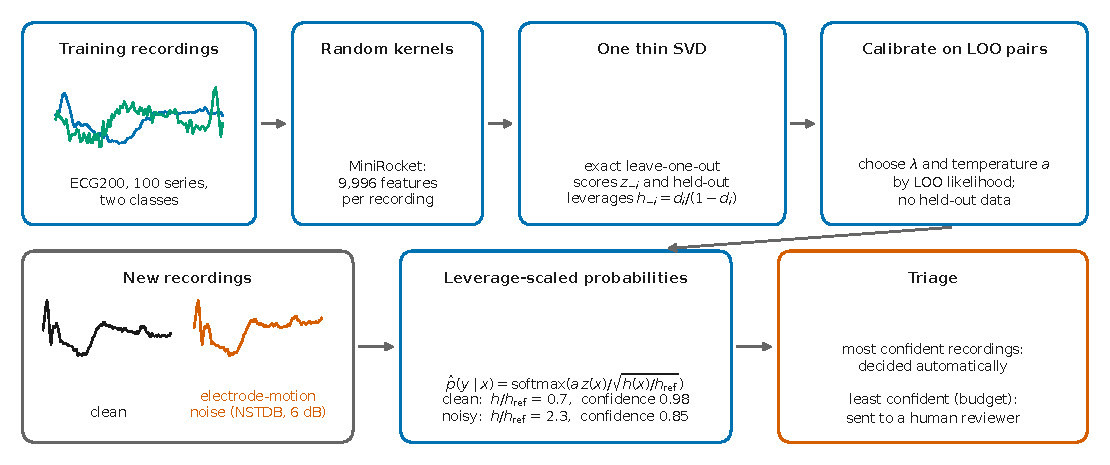
\includegraphics[width=\textwidth]{fig_schematic.pdf}
\caption{LOOM turns the ridge readout of a random-kernel classifier into probabilities whose confidence drops for unusual recordings. Examples are real: the first training series of each class of ECG200 and the first test series in file order, shown clean and with real electrode-motion noise from the MIT-BIH Noise Stress Test Database at 6\,dB; the printed leverage ratios and confidences are computed by the fitted model.}\label{fig:schematic}
\end{figure*}

\begin{algorithm}[t]
\caption{LOOM: fitting and triage}\label{alg:loom}
\begin{algorithmic}[1]
\Require training series $\{(x_i,y_i)\}_{i=1}^n$, penalty grid $\Lambda$, review budget $b$
\State Fit the random-kernel transform; compute standardised features $\psi(x_i)$
\State Thin SVD $\Phi_c=USV^\top$ \Comment{one decomposition for all $\lambda$}
\For{$\lambda\in\Lambda$}
  \State $d_i$ by Eq.~\eqref{eq:leverage}; $z_{-i}$ and $h_{-i}$ by Eq.~\eqref{eq:loo}; $h_{\mathrm{ref}}\gets\mathrm{median}(h_{-i})$
  \State $a_\lambda\gets\arg\min_a\mathcal L(a,\lambda)$ by Eq.~\eqref{eq:fit} with smoothed targets
\EndFor
\State $(\lambda^\star,a^\star)\gets\arg\min_\lambda \mathcal L(a_\lambda,\lambda)$
\For{each new recording $x$}
  \State $\hat p(\cdot\mid x)$ by Eq.~\eqref{eq:loom} with $\lambda^\star,a^\star$; optional jackknife+ set by Eq.~\eqref{eq:jk}
\EndFor
\State Send the $b$ share of recordings with the lowest $\max_k\hat p(k\mid x)$ to review; decide the rest automatically
\end{algorithmic}
\end{algorithm}

\subsection{Exact leave-one-out scores and held-out leverages}
Let $B_{-i}$ denote the fit without example $i$ (same $\lambda$ and standardisation).
\begin{proposition}[LOO scores and held-out leverages]\label{prop:loo}
\begin{equation}\label{eq:loo}
z_{-i}:=B_{-i}^\top\tilde x_i=Y_i-\frac{Y_i-\hat Y_i}{1-d_i},\qquad h_{-i}:=\tilde x_i^\top A_{-i}^{-1}\tilde x_i=\frac{d_i}{1-d_i}.
\end{equation}
\end{proposition}
The first identity is the classical PRESS shortcut \citep{allen1974} used by RidgeClassifierCV and PreVal; the second follows from the same Sherman--Morrison update and is the quantity LOOM adds. Proofs are in Supplementary Sect.~\ref{S-sec:proofs}. The pair $(z_{-i},h_{-i})$ is an exact out-of-sample observation of a score and its uncertainty, available for all $n$ examples at $O(nr)$ cost.

\subsection{Leverage-scaled probabilities}
Under the Bayesian linear model with prior $\beta\sim\mathcal N(0,\sigma^2\lambda^{-1}I)$, the predictive standard deviation of each score is $\sigma\sqrt{h(x)}$. LOOM divides the scores by this quantity relative to $h_{\mathrm{ref}}=\mathrm{median}(h_{-i})$:
\begin{equation}\label{eq:loom}
\hat p(y=k\mid x)=\mathrm{softmax}_k\!\left(\frac{a\,z_k(x)}{\sqrt{h(x)/h_{\mathrm{ref}}}}\right).
\end{equation}
The leverage is a ridge-regularised Mahalanobis distance of $\psi(x)$ from the training mean, plus $1/n$, computed in the geometry the classifier itself uses. For recordings like the training data $h(x)\approx h_{\mathrm{ref}}$ and Eq.~\eqref{eq:loom} is a temperature-scaled ridge; when a fault moves a recording away from the training span, $h(x)$ grows and the probabilities move towards uniform. Eq.~\eqref{eq:loom} is the limit $c\to\infty$ of the moderation $\mathrm{softmax}\big(az/\sqrt{1+ch/h_{\mathrm{ref}}}\big)$ \citep{kristiadi2020,mackay1992}; the limit was fixed on eight development datasets before the benchmark, and finite $c$ is an ablation.

\subsection{Fitting on exact LOO pairs}
For each $\lambda$ the temperature minimises the LOO negative log-likelihood
\begin{equation}\label{eq:fit}
\mathcal L(a,\lambda)=-\frac1n\sum_{i=1}^n\sum_{k=1}^K t_{ik}\log\mathrm{softmax}_k\!\left(\frac{a\,z_{-i,k}}{\sqrt{h_{-i}/h_{\mathrm{ref}}}}\right),
\end{equation}
and the pair $(\lambda,a)$ with the smallest value is kept. When the LOO predictions separate the classes, the optimal temperature is infinite; we therefore smooth the targets following \citet{platt1999}: the true class receives $(n_k+1)/(n_k+2)$, where $n_k$ is its training count, and the rest is spread evenly. The one-dimensional problem in $\log a$ is solved with L-BFGS from three starting values.

\subsection{Closed-form jackknife+ prediction sets}\label{sec:jackknife}
With a non-conformity score $s(x,y;f)$ (LAC, $1-\hat p(y\mid x)$ \citep{sadinle2019}, or deterministic APS \citep{romano2020}), jackknife+ returns $C(x)=\{y:\#\{i:s_i<s(x,y;f_{-i})\}<(1-\alpha)(n+1)\}$ with $s_i=s(x_i,y_i;f_{-i})$ \citep{barber2021}. It needs every LOO model at every test point.
\begin{proposition}[LOO predictions at a new point]\label{prop:jk}
With $k(x,i)=\tilde x(x)^\top A^{-1}\tilde x_i=1/n+(V^\top\psi)^\top D_\lambda S u_i$ and residuals $E=Y-\hat Y$,
\begin{equation}\label{eq:jk}
z_{-i}(x)=z(x)-\frac{k(x,i)E_i}{1-d_i},\qquad h_{-i}(x)=h(x)+\frac{k(x,i)^2}{1-d_i}.
\end{equation}
\end{proposition}
This parallels closed-form conformal ridge regression \citep{nouretdinov2001}. Because $\lambda$, $a$ and the standardisation use all $n$ examples (Assumption~\ref{as:fixed}), the coverage guarantee holds only approximately; we check it empirically (Sect.~\ref{sec:validity}).

\subsection{Complexity}
The SVD costs $O(np\min(n,p))$, as for RidgeClassifierCV; ten penalties and the temperature fits add $O(10\,nrK)$; prediction costs $O(p(r+K))$ per series instead of $O(pK)$; memory is $O((n+p)r)$. Cross-validated calibration needs $k$ further fits and an $M$-member ensemble $M$ transforms and fits.

%=====================================================================
\section{Experimental framework}\label{sec:framework}

\subsection{Setup}
Code is in Python (NumPy, SciPy, scikit-learn \citep{pedregosa2011}, aeon 1.6.0 \citep{aeon2024}). Every job ran on one core of a 4-core cloud CPU without a GPU (14.3\,GB memory limit); times are single-core wall-clock times. One script regenerates all results, tables, figures and the number macros of this paper; unit tests compare Eqs.~\eqref{eq:leverage}, \eqref{eq:loo} and \eqref{eq:jk} with explicit refits. The method was developed on eight datasets and the pipeline tested on six more; results without them are reported. The protocol was registered before the benchmark, and every later change is logged (Supplementary Sect.~\ref{S-sec:deviations}). An AI assistant (Claude, Anthropic) was used for the literature search, for writing and running code and for drafting text; all numbers come from the released result files, and the authors take responsibility for the content.

\subsection{Datasets}
Table~\ref{tab:datasets} lists the data. The benchmark uses the \NDatasets{} univariate equal-length UCR datasets \citep{dau2019ucr} with the official split and four stratified resamples (three for the four largest datasets), following the bake-off protocol \citep{bagnall2017bakeoff}. A leakage audit found exact train/test duplicates in \NDupExact{} datasets and exact or near duplicates in \NDupNear{}; a planted-leak test confirmed that the audit detects such cases (Supplementary Sect.~\ref{S-sec:leakage}).

\begin{table}[t]
\caption{Data used in each experiment. All datasets are from the UCR archive; real noise is from the MIT-BIH Noise Stress Test Database.}\label{tab:datasets}
\centering\footnotesize
\begin{tabular}{P{2.8cm}P{3.6cm}P{2.4cm}P{3.4cm}}
\toprule
Experiment & Datasets & Splits & Purpose \\
\midrule
Benchmark (E1--E9) & \NDatasets{} univariate, equal length & official + 4 resamples & calibration, faults, ablation, prediction sets \\
Real ECG noise (E12) & 7 ECG datasets & official + 4 resamples & real recorded noise, 9 conditions \\
Triage, exploratory (E11) & 12 sensor datasets, 3 domains & official + 4 resamples & review-queue study \\
Triage, confirmatory (E13) & \CNDatasets{} further sensor datasets & official + 4 resamples & pre-registered replication \\
QUANT features (E14) & \QFN{} datasets ($\le$ 3{,}000 training series) & official split & non-convolutional features \\
Natural change (E10) & UWaveGestureLibrary X/Y/Z & official + 4 resamples & cross-axis sensor change \\
\bottomrule
\end{tabular}
\end{table}

\subsection{Faults and the triage protocol}\label{sec:faultsetup}
\emph{Simulated faults} are applied to test series only, with amplitudes relative to each series' standard deviation: noise, baseline wander or drift, dropout (a segment replaced by interpolation), spikes, speed variation (smooth time warp) and misalignment (circular shift), each at three severities (Supplementary Sect.~\ref{S-sec:faults}). \emph{Real noise}: baseline wander, electrode motion and muscle artefact recordings of the MIT-BIH Noise Stress Test Database \citep{goldberger2000physionet,moody1984nstdb} are added at 12, 6 and 0\,dB SNR to the seven ECG datasets. \emph{Triage}: each test recording is faulty with probability 0.3, with a domain-specific fault at a random severity; the share $b$ of recordings with the lowest confidence goes to review.

\subsection{Metrics}
With predicted probabilities $\hat p_{ik}$ and true labels $y_i$ on $m$ test recordings, we report the negative log-likelihood, the expected calibration error over 15 equal-width bins $B_1,\dots,B_{15}$ of the top-label confidence, and the Brier score:
\begin{align}
\mathrm{NLL}&=-\frac1m\sum_{i}\log\hat p_{iy_i},\qquad
\mathrm{Brier}=\frac1m\sum_{i,k}\big(\hat p_{ik}-\mathbb 1[y_i=k]\big)^2,\\
\mathrm{ECE}&=\sum_{j}\frac{|B_j|}{m}\big|\mathrm{acc}(B_j)-\mathrm{conf}(B_j)\big| .
\end{align}
Fault detection is measured by the AUROC of $1-\max_k\hat p_{ik}$ for separating faulty from clean recordings. For prediction sets we report coverage $\frac1m\sum_i\mathbb 1[y_i\in C(x_i)]$ and mean set size. For triage with review set $R$ ($|R|=bm$) and faulty set $F$:
\begin{equation}
\text{faults caught}=\frac{|R\cap F|}{|F|},\qquad
\text{automatic error}=\frac{|\{i\notin R:\hat y_i\neq y_i\}|}{m-|R|}.
\end{equation}

\subsection{Baselines}
All readouts use identical MiniRocket features: ridge one-hot output, softmax of the ridge scores, PreVal \citep{dempster2025preval} (reimplemented without smoothing, as published), hold-out temperature scaling (80/20), five-fold Platt and isotonic calibration \citep{pedregosa2011}, cross-validated logistic regression, and five-seed ensembles of PreVal and LOOM. QUANT \citep{dempster2024quant} and the Arsenal \citep{middlehurst2021hc2} work on the raw series. Eight ablations remove or replace one component of LOOM at a time (Sect.~\ref{sec:ablation}). All methods receive the same data, seeds and fixed hyperparameter grids.

\subsection{Hypotheses and tests}
Table~\ref{tab:hyp} lists the hypotheses with their metrics and outcomes. Datasets are the unit of analysis, with each metric averaged over resamples. We use two-sided Wilcoxon signed-rank tests \citep{wilcoxon1945} with Holm's correction \citep{holm1979}, as recommended for comparisons across datasets \citep{benavoli2016,demsar2006}, report how many datasets a result holds in, means with 95\,\% bootstrap confidence intervals (1{,}000 resamples), and Bayesian signed-rank tests \citep{benavoli2017bayesian} with a region of practical equivalence of $\pm0.01$ nats for NLL and $\pm1$ percentage point for rates. Only the hypotheses in Table~\ref{tab:hyp} are confirmatory; all other comparisons are descriptive, with Holm's correction applied within each table. Numeric pass criteria for H1--H3 were written down after the results (deviation D18).

%=====================================================================
\section{Results and analysis}\label{sec:results}

\subsection{Hypothesis tests}\label{sec:hyp}
Table~\ref{tab:hyp} summarises the outcomes and Fig.~\ref{fig:main} the main comparison. Of the \NHyp{} pre-specified hypotheses, \NHypPass{} passed and \HypFailed{} failed.

\begin{table*}[t]
\caption{Hypotheses, tests and outcomes. H1--H3 were registered on 13 October 2026 before the benchmark, H4--H7 on 2 November 2026 before the corresponding experiments (Supplementary Sect.~\ref{S-sec:deviations}). Counts give the datasets (or dataset--noise combinations) in favour of LOOM; $p$ is Holm-adjusted.}\label{tab:hyp}
\centering\footnotesize
\begin{tabular}{P{0.6cm}P{4.0cm}P{1.6cm}P{4.6cm}l}
\toprule
ID & Hypothesis & Metric & Result & Outcome \\
\midrule
H1a & Clean NLL not worse than PreVal, hold-out TS, Platt, LogReg & NLL & vs PreVal: not significantly different, with 49 wins and 65 losses of 114 datasets, $p=1.000$ & pass \\
H1b & Clean ECE and Brier not worse than PreVal & ECE, Brier & ECE: LOOM worse on 86 of 114 datasets, $p<0.001$ & \textbf{fail} \\
H1c & Accuracy unchanged vs PreVal & accuracy & not significantly different, with 28 wins and 29 losses of 114 datasets, $p=0.572$ & pass \\
H2a & Faults: NLL lower than every closed-form / CV readout & NLL, 18 conditions & vs PreVal: LOOM better on 108/114, $p<0.001$; all 7 readouts & pass \\
H2b & Faults: better detection of faulty inputs than PreVal & AUROC & LOOM better on 114/114, $p<0.001$ & pass \\
H3 & Jackknife+: coverage 0.88--0.92, smaller sets than split & coverage, size & coverage 0.898; smaller on 103/114, $p<0.001$ & pass \\
H4 & Real ECG noise: NLL lower than PreVal & NLL, 63 cells & LOOM better on 50/63, $p<0.001$ & pass \\
H5 & Triage: more faulty recordings caught than PreVal & 20\,\% budget & LOOM better on 38/38, $p<0.001$ & pass \\
H6 & Triage: fewer automatic errors than PreVal & 20\,\% budget & LOOM better on 35/38, $p<0.001$ & pass \\
H7 & QUANT features: NLL under faults lower than PreVal & NLL, severity 3 & LOOM better on 110/110, $p<0.001$ & pass \\
\bottomrule
\end{tabular}

\end{table*}

\begin{figure*}[t]
\centering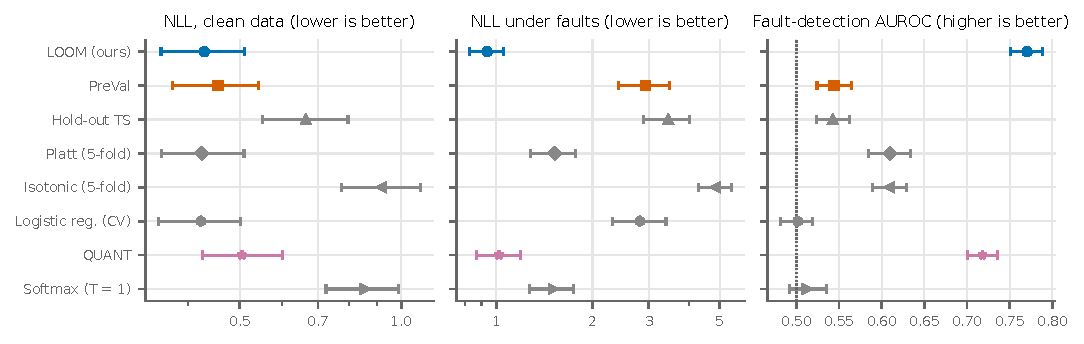
\includegraphics[width=\textwidth]{fig_main_results.pdf}
\caption{LOOM is on a par with the best readouts on clean data and clearly better than the other readouts under simulated faults, where QUANT is close to it. Means over the \NDatasets{} UCR datasets of the per-dataset mean over resamples, with 95\,\% bootstrap confidence intervals: NLL on clean data, NLL averaged over 18 simulated fault conditions (log scale), and AUROC for detecting faulty recordings. Ridge one-hot is omitted because its NLL is off scale.}\label{fig:main}
\end{figure*}

\subsection{Calibration on clean data (H1)}\label{sec:clean}
On clean data LOOM is roughly on a par with the best readouts but not better (Table~\ref{tab:clean}). Its median NLL is \NLLCleanLoom; compared with PreVal it is \CmpNLLCleanPreVal, and it is also not significantly different from five-fold Platt scaling and logistic regression. A non-significant test does not mean equivalence: the Bayesian analysis gives probability \BayesCleanPreValBetter{} that LOOM is better, \BayesCleanPreValEquiv{} that the two are practically equivalent and \BayesCleanPreValWorse{} that PreVal is better, and the per-dataset differences exceed resampling noise in favour of PreVal on \NoiseCleanPreVal{} of the datasets and in favour of LOOM on \NoiseCleanLoom{} (Sect.~\ref{sec:sanity}). LOOM's calibration error is higher than PreVal's (median ECE \ECECleanLoom{} vs \ECECleanPreVal; LOOM \CmpECECleanPreVal), and so is its Brier score; H1b therefore fails. The cause is the target smoothing (Sect.~\ref{sec:ablation}). Accuracy is the same as PreVal's (median \AccCleanLoom{} vs \AccCleanPreVal).

\begin{table}[t]
\caption{Clean test data, \NDatasets{} datasets: median over datasets of the mean over resamples. W/D/L counts datasets on which LOOM is better/equal/worse in NLL; $p$ is the Holm-adjusted Wilcoxon $p$-value for NLL.}\label{tab:clean}
\centering\scriptsize
\begin{tabular}{lrrrrrr}
\toprule
Method & NLL & ECE & Brier & Acc. & W/D/L & $p$ \\
\midrule
LOOM (ours) & 0.295 & 0.075 & 0.144 & 0.914 & -- & -- \\
PreVal & 0.360 & 0.040 & 0.134 & 0.914 & 49/0/65 & $p=1.000$ \\
Hold-out TS & 0.524 & 0.052 & 0.177 & 0.896 & 85/0/29 & $p<0.001$ \\
Ridge + Platt (5-fold) & 0.294 & 0.080 & 0.148 & 0.912 & 53/0/57 & $p=1.000$ \\
Ridge + isotonic (5-fold) & 0.670 & 0.044 & 0.157 & 0.904 & 96/0/14 & $p<0.001$ \\
Logistic regression (CV) & 0.314 & 0.049 & 0.151 & 0.901 & 53/0/56 & $p=1.000$ \\
QUANT & 0.386 & 0.116 & 0.210 & 0.895 & 77/0/37 & $p<0.001$ \\
Ridge softmax ($T=1$) & 0.588 & 0.249 & 0.284 & 0.914 & 110/0/4 & $p<0.001$ \\
Ridge one-hot & 2.959 & 0.086 & 0.171 & 0.914 & 103/0/11 & $p<0.001$ \\
\bottomrule
\end{tabular}

\end{table}

\subsection{Simulated sensor faults (H2)}\label{sec:faults}
The leverage reacts to faults (Fig.~\ref{fig:leverage}). For clean test series the median ratio $h(x)/h_{\mathrm{ref}}$ is \LevClean; at the highest severity it reaches \LevNoise{} for noise, \LevSpikes{} for spikes, \LevMissing{} for dropout, \LevWander{} for baseline wander and \LevShift{} for misalignment, but only \LevWarp{} for speed variation. Averaged over the 18 conditions (Table~\ref{tab:faults}), LOOM's median NLL is \NLLFaultsLoom{} against \NLLFaultsPreVal{} for PreVal; LOOM is \CmpNLLFaultsPreVal{} (Bayesian probability \BayesFaultsPreValBetter{} that LOOM is better; mean NLL with 95\,\% CI \CINLLFaultsLoom{} vs \CINLLFaultsPreVal), and it is also better than hold-out, Platt and isotonic calibration and logistic regression. Accuracy is unchanged (median \AccFaultsLoom{} vs \AccFaultsPreVal): the gain comes from lower confidence on the damaged recordings that are misclassified. The median AUROC for detecting faulty recordings is \AUROCFaultsLoom{} for LOOM and \AUROCFaultsPreVal{} for PreVal. Figure~\ref{fig:robust} shows that the gap grows with severity for every fault type except speed variation.

\begin{figure}[t]
\centering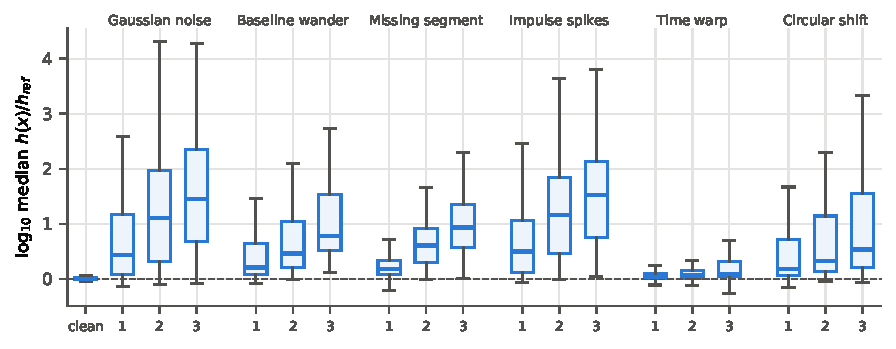
\includegraphics[width=\columnwidth]{fig_leverage_ratio.pdf}
\caption{Faults push recordings away from the training data, except speed variation. Distribution over datasets of the median leverage ratio $h(x)/h_{\mathrm{ref}}$ ($\log_{10}$) for clean data and each simulated fault at severities 1--3.}\label{fig:leverage}
\end{figure}

\begin{table}[t]
\caption{Simulated faults, \NDatasets{} datasets: per-dataset mean over 18 conditions, then median over datasets. Statistics as in Table~\ref{tab:clean}.}\label{tab:faults}
\centering\scriptsize
\begin{tabular}{lrrrrrr}
\toprule
Method & NLL & ECE & Acc. & AUROC & W/D/L & $p$ \\
\midrule
LOOM (ours) & 0.738 & 0.151 & 0.695 & 0.765 & -- & -- \\
PreVal & 1.728 & 0.185 & 0.692 & 0.563 & 108/0/6 & $p<0.001$ \\
Hold-out TS & 2.221 & 0.197 & 0.676 & 0.558 & 110/0/4 & $p<0.001$ \\
Ridge + Platt (5-fold) & 1.125 & 0.144 & 0.697 & 0.610 & 86/0/24 & $p<0.001$ \\
Ridge + isotonic (5-fold) & 4.358 & 0.153 & 0.682 & 0.592 & 108/0/2 & $p<0.001$ \\
Logistic regression (CV) & 1.878 & 0.219 & 0.660 & 0.516 & 104/0/5 & $p<0.001$ \\
QUANT & 0.732 & 0.170 & 0.694 & 0.709 & 44/0/70 & $p=0.291$ \\
Ridge softmax ($T=1$) & 1.086 & 0.256 & 0.696 & 0.531 & 105/0/9 & $p<0.001$ \\
Ridge one-hot & 10.495 & 0.304 & 0.696 & 0.500 & 114/0/0 & $p<0.001$ \\
\bottomrule
\end{tabular}

\end{table}

\begin{figure*}[t]
\centering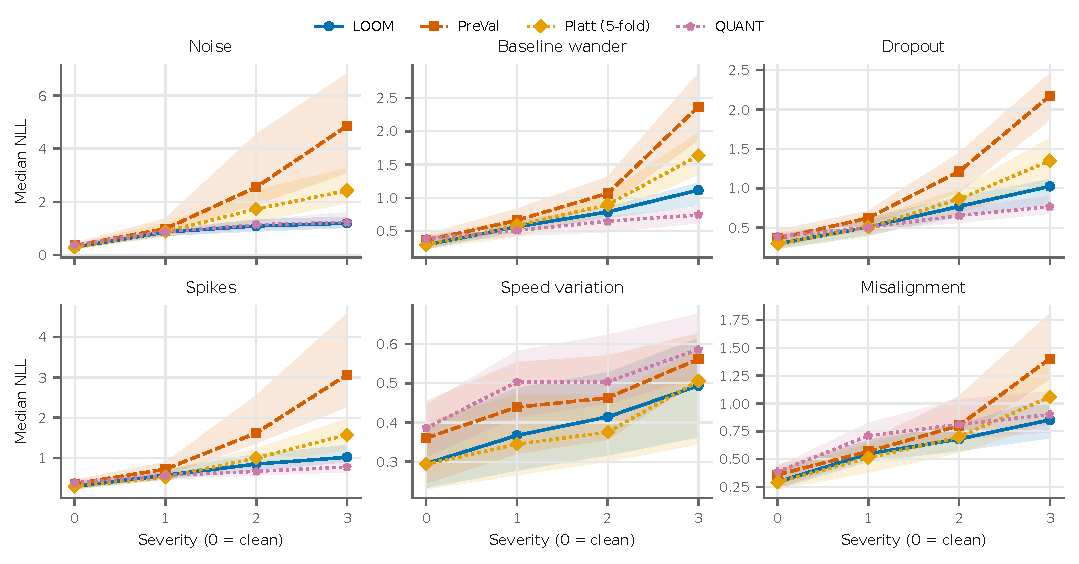
\includegraphics[width=\textwidth]{fig_robustness.pdf}
\caption{LOOM's advantage over PreVal grows with fault severity, but QUANT is better for baseline wander, dropout and spikes at the highest severity. Median NLL over the \NDatasets{} datasets against severity for each simulated fault, with 95\,\% bootstrap bands of the median.}\label{fig:robust}
\end{figure*}

\subsection{Real-world validation: recorded ECG noise (H4)}\label{sec:realnoise}
Figure~\ref{fig:realnoise} and Table~\ref{tab:realnoise} show the results with real noise. All methods have a similar NLL on the clean ECG recordings (median \RNCleanNLLLoom{} for LOOM, \RNCleanNLLPreVal{} for PreVal). With real noise added, PreVal's median NLL rises to \RNNLLPreVal{} and LOOM's to \RNNLLLoom. Over the \RNNCells{} combinations of dataset, noise type and level, LOOM compared with PreVal is \CmpRNCellsPreVal, which confirms H4 (Bayesian probability \BayesRealNoisePreValBetter{} that LOOM is better); compared with QUANT it is \CmpRNCellsQuant. LOOM recognises noisy recordings best: its median detection AUROC is \RNAUROCLoom, against \RNAUROCQuant{} for QUANT (LOOM \CmpRNAUROCCellsQuant) and \RNAUROCPreVal{} for PreVal. In a stream with 30\,\% noisy recordings and a 20\,\% review budget, LOOM's queue contains \RNCaughtLoom{} of the noisy recordings, against \RNCaughtPreVal{} for PreVal and \RNCaughtQuant{} for QUANT, while QUANT has the lowest automatic error rate (\RNErrQuant{} vs \RNErrLoom{} for LOOM). With seven datasets, dataset-level tests have little power; the conclusions rest on the 63 combinations.

\begin{figure*}[t]
\centering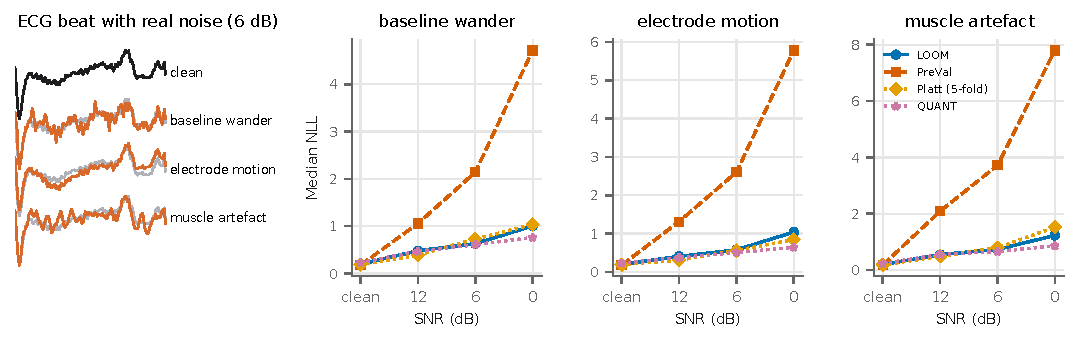
\includegraphics[width=\textwidth]{fig_real_noise.pdf}
\caption{Under real recorded ECG noise, PreVal's NLL explodes while LOOM's stays close to QUANT's. Left: an ECG5000 beat (grey) with each MIT-BIH NSTDB noise type at 6\,dB (orange). Right: median NLL over the seven ECG datasets against signal-to-noise ratio for each noise type.}\label{fig:realnoise}
\end{figure*}

\begin{table}[t]
\caption{Real recorded ECG noise on seven ECG datasets: median over datasets. Noisy NLL, detection AUROC and accuracy average nine combinations of noise type and SNR; ``Caught'' and ``Auto err.'' refer to a stream with 30\,\% noisy recordings and a 20\,\% review budget.}\label{tab:realnoise}
\centering\scriptsize
\begin{tabular}{lrrrrrr}
\toprule
Method & Clean NLL & Noisy NLL & AUROC & Acc. & Caught & Auto err. \\
\midrule
LOOM (ours) & 0.196 & 0.678 & 0.973 & 0.684 & 63\,\% & 7.5\,\% \\
PreVal & 0.175 & 3.346 & 0.591 & 0.673 & 34\,\% & 9.2\,\% \\
Hold-out TS & 0.194 & 6.097 & 0.623 & 0.675 & 37\,\% & 10.2\,\% \\
Ridge + Platt (5-fold) & 0.186 & 0.686 & 0.737 & 0.686 & 44\,\% & 9.0\,\% \\
QUANT & 0.231 & 0.585 & 0.899 & 0.700 & 49\,\% & 4.8\,\% \\
\bottomrule
\end{tabular}

\end{table}

\subsection{Case study: triage of faulty recordings (H5, H6)}\label{sec:triage}
In the exploratory study (12 datasets, 20\,\% review budget), LOOM's review queue contained a median of \XCaughtLoom{} of the faulty recordings, against \XCaughtPreVal{} for PreVal and \XCaughtQuant{} for QUANT, and caught more than PreVal on all twelve datasets (\XCaughtPPreVal). Its automatic error rate was lower in the median (\XErrLoom{} vs \XErrPreVal) but not significantly (\XErrPPreVal), and QUANT made the fewest automatic errors (\XErrQuant).

The pre-registered confirmatory replication on \CNDatasets{} further datasets (Fig.~\ref{fig:triage}, Table~\ref{tab:triage}) confirmed both hypotheses under Holm's correction over all eight primary tests. LOOM's queue caught a median of \CCaughtLoom{} of the faulty recordings, against \CCaughtPreVal{} for PreVal (LOOM \CmpCCaughtPreVal; H5) and \CCaughtQuant{} for QUANT (LOOM \CmpCCaughtQuant). Its automatic error rate was \CErrLoom, against \CErrPreVal{} for PreVal (LOOM \CmpCErrPreVal; H6) and \CErrQuant{} for QUANT (LOOM \CmpCErrQuant). Means with 95\,\% CIs are \CICCaughtLoom{} (LOOM) and \CICCaughtPreVal{} (PreVal) for faults caught. The advantage over PreVal remains after merging datasets from the same source (LOOM \CmpCCaughtGrouped). On fault-free streams the methods behave alike (automatic error \CErrCleanLoom{} vs \CErrCleanPreVal), so LOOM does not change how a system behaves on good data. A post hoc check (deviation D22) reduced the share of faulty recordings by subsampling the stored outputs: at 10\,\% prevalence LOOM's queue caught \PrevTenCaughtLoom{} against \PrevTenCaughtPreVal{} for PreVal (LOOM \CmpPrevTenCaughtPreVal) and its automatic error was \PrevTenErrLoom{} against \PrevTenErrPreVal{} (LOOM \CmpPrevTenErrPreVal). For an operator, this means that with one recording in five sent to review, about \CCaughtLoom{} instead of \CCaughtPreVal{} of the damaged recordings reach a person.

\begin{figure*}[t]
\centering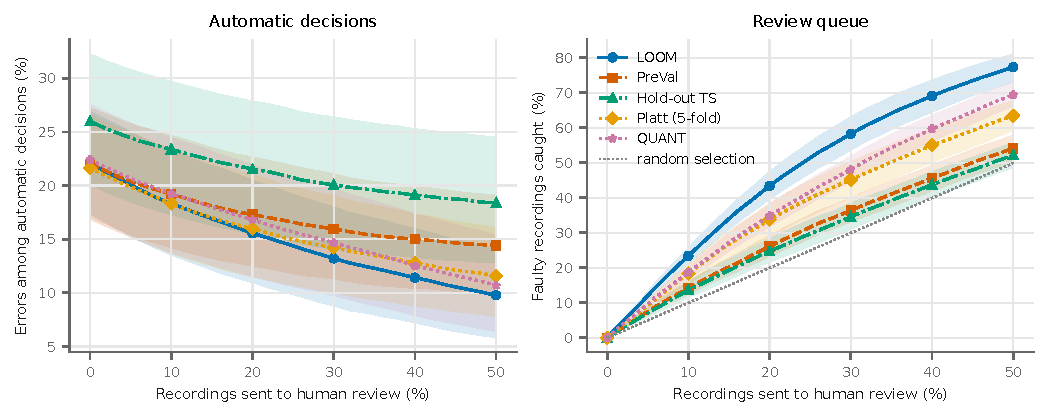
\includegraphics[width=\textwidth]{fig_triage.pdf}
\caption{In the pre-registered triage study, LOOM's review queue catches the most faulty recordings at every budget. \CNDatasets{} sensor datasets with 30\,\% faulty recordings: error rate of automatic decisions (left) and share of faulty recordings caught (right) against the review budget; means over datasets of the mean over resamples with 95\,\% bootstrap bands over datasets (bands include the differences in difficulty between datasets; paired comparisons are in the text).}\label{fig:triage}
\end{figure*}

\begin{table}[t]
\caption{Triage with a 20\,\% review budget: median over datasets of the share of faulty recordings caught and of the error rate of automatic decisions, in the exploratory (12 datasets) and confirmatory (\CNDatasets{} datasets) studies, and the automatic error on fault-free streams (confirmatory).}\label{tab:triage}
\centering\scriptsize
\begin{tabular}{lrrrrr}
\toprule
& \multicolumn{2}{c}{Exploratory (12)} & \multicolumn{3}{c}{Confirmatory (\CNDatasets)} \\ \cmidrule(lr){2-3}\cmidrule(lr){4-6}
Method & Caught & Auto err. & Caught & Auto err. & No faults \\
\midrule
LOOM (ours) & 45\,\% & 4.2\,\% & 41\,\% & 10.1\,\% & 4.4\,\% \\
PreVal & 25\,\% & 9.5\,\% & 24\,\% & 14.6\,\% & 4.8\,\% \\
Hold-out TS & 26\,\% & 9.9\,\% & 23\,\% & 19.8\,\% & 9.8\,\% \\
Ridge + Platt (5-fold) & 27\,\% & 8.7\,\% & 28\,\% & 15.0\,\% & 4.6\,\% \\
QUANT & 38\,\% & 1.6\,\% & 34\,\% & 13.2\,\% & 8.9\,\% \\
\bottomrule
\end{tabular}

\end{table}

\subsection{Comparative analysis: ensembles, raw-series classifiers and QUANT features (H7)}\label{sec:comparative}
On the official split (Table~\ref{tab:official}) the comparison under faults uses the six severity-3 conditions for every method, because the Arsenal was only run there; this restriction was introduced after the results were first inspected and works against LOOM (deviation D10). On clean data a five-seed PreVal ensemble is slightly better than a single LOOM model (LOOM \CmpNLLOffCleanPreValEns), while LOOM beats QUANT (LOOM \CmpNLLOffCleanQuant). Under the strongest faults LOOM beats the PreVal ensemble and the Arsenal, but QUANT is better (LOOM \CmpNLLOffSevThreeQuant); averaged over all 18 conditions the two do not differ significantly (Table~\ref{tab:faults}), but the Bayesian probability that QUANT is better is \BayesFaultsQuantWorse. At the highest severity QUANT has the lower median NLL for \FamQuantBetter, and LOOM for \FamLoomBetter. The Arsenal's high NLL comes mainly from vote-based probabilities that give exactly zero to the true class; in the bounded Brier score the clean gap is small (\BrierOffCleanArsenal{} vs \BrierOffCleanLoom).

To see whether QUANT's robustness comes from its features or its trees, we fitted the readouts on QUANT's features (median \QFFeatures{} features, \QFN{} datasets). LOOM again rescued the ridge readout under faults: PreVal's median NLL was \QFNLLFaultsPreValQF{} and LOOM's \QFNLLFaultsLoom{} (LOOM \CmpQFPreVal), confirming H7. LOOM on QUANT features also detected faults far better than the QUANT classifier (AUROC \QFAUROCLoom{} vs \QFAUROCQuant; LOOM \CmpQFAUROCQuant). But the linear readout lost much more accuracy than QUANT's trees (\QFAccLoom{} vs \QFAccQuant), so QUANT kept the lower NLL (LOOM \CmpQFQuant). QUANT's robustness therefore comes mainly from its trees, whose outputs stay within the range seen in training, while LOOM's strength is recognising unusual inputs; the two are complementary.

\begin{table}[t]
\caption{Official split, strongest (severity-3) simulated faults: median over datasets. Statistics as in Table~\ref{tab:clean}. The Arsenal has no result on Fungi (undefined probabilities with one training series per class).}\label{tab:official}
\centering\scriptsize
\begin{tabular}{lrrrrrr}
\toprule
Method & NLL & Brier & Acc. & AUROC & W/D/L & $p$ \\
\midrule
LOOM (ours) & 1.020 & 0.526 & 0.604 & 0.845 & -- & -- \\
LOOM, 5-seed ens. & 1.003 & 0.519 & 0.614 & 0.847 & 38/0/76 & $p<0.001$ \\
PreVal & 2.260 & 0.673 & 0.613 & 0.531 & 105/0/9 & $p<0.001$ \\
PreVal, 5-seed ens. & 2.040 & 0.636 & 0.616 & 0.584 & 104/0/10 & $p<0.001$ \\
QUANT & 0.931 & 0.489 & 0.621 & 0.760 & 36/0/78 & $p=0.042$ \\
Arsenal & 7.024 & 0.672 & 0.600 & 0.676 & 110/0/3 & $p<0.001$ \\
\bottomrule
\end{tabular}

\end{table}

\subsection{Ablation study}\label{sec:ablation}
Figure~\ref{fig:ablation} compares LOOM with eight variants. Removing the leverage scaling while keeping smoothing (PreVal-smooth) is much worse under faults (median NLL \NLLAblFaultsPreValSmooth{} vs \NLLAblFaultsLoom; LOOM \CmpNLLAblFaultsPreValSmooth), while on clean data LOOM is \CmpNLLAblCleanPreValSmooth, so the scaling has a small cost on clean data. Calibrating on in-sample instead of LOO pairs gives a median clean NLL of \NLLAblCleanInSample, and an 80/20 split \NLLAblCleanHoldoutPairs, so the exact LOO pairs matter. A finite moderation strength ($c=1$) gives a slightly lower clean NLL (LOOM \CmpNLLAblCleanFiniteC) but detects faults worse (AUROC \AUROCAblFaultsFiniteC{} vs \AUROCAblFaultsLoom; LOOM higher on \NWinsAUROCFiniteC{} of \NDatasets{} datasets). Removing the smoothing brings the clean ECE to PreVal's level (\ECEAblCleanNoSmooth{} vs \ECEAblCleanPreVal) but is worse under faults (LOOM \CmpNLLAblFaultsNoSmooth). A nearest-neighbour distance in place of leverage gives similar NLL but worse detection (AUROC \AUROCAblFaultsKNN).

\begin{figure*}[t]
\centering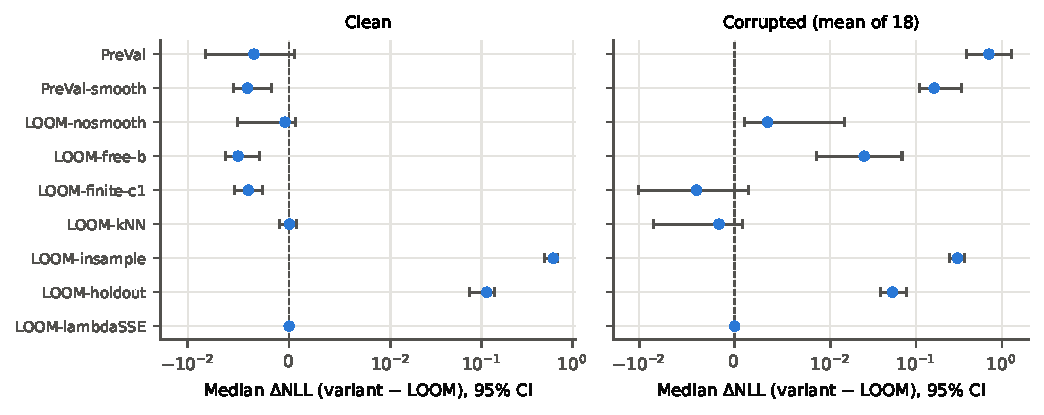
\includegraphics[width=\textwidth]{fig_ablation.pdf}
\caption{The leverage scaling and the exact LOO pairs are what make LOOM work under faults. Median paired NLL difference (variant $-$ LOOM) over the \NDatasets{} datasets with bootstrap 95\,\% confidence intervals, clean data (left) and simulated faults (right); positive values mean that the variant is worse.}\label{fig:ablation}
\end{figure*}

\subsection{Prediction sets and validity (H3)}\label{sec:validity}
On clean data LOOM's closed-form jackknife+ sets with the LAC score cover \CPLoomCovClean{} of test series at target 0.9 with \CPLoomSizeClean{} labels per set, against \CPSplitCovClean{} and \CPSplitSizeClean{} for split conformal prediction (set size \CmpSetSizeSplit), so H3 passes (Fig.~\ref{fig:validity}a, Table~\ref{S-tab:conformal}). Coverage at targets 0.95 and 0.8 is \CPLoomCovAlphaFive{} and \CPLoomCovAlphaTwenty. Under faults coverage drops because damaged recordings are not exchangeable with training data (Fig.~\ref{fig:validity}b); with LAC, LOOM's flat probabilities produce empty sets for \CPLoomEmptyFaults{} of damaged recordings, whereas APS keeps coverage at \CPLoomAPSCovFaults. The reliability diagrams (Fig.~\ref{fig:validity}c) show that LOOM stays close to the diagonal under strong faults while PreVal becomes overconfident.

\begin{figure*}[t]
\centering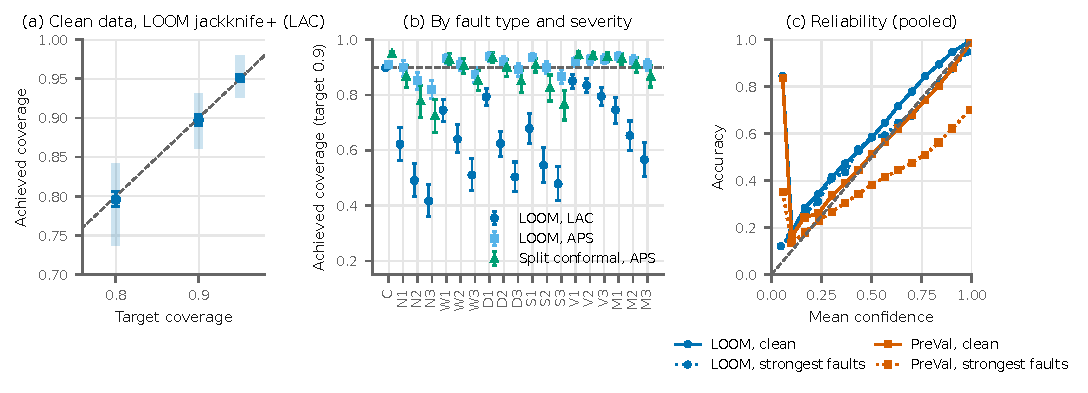
\includegraphics[width=\textwidth]{fig_validity.pdf}
\caption{Jackknife+ coverage matches its target on average on clean data; under faults only APS sets keep coverage. (a) Target vs achieved coverage of LOOM's jackknife+ sets (LAC), mean over datasets with 95\,\% bootstrap CI and 10th--90th percentile of datasets (band). (b) Achieved coverage at target 0.9 by condition (C clean; N noise, W baseline wander, D dropout, S spikes, V speed variation, M misalignment; 1--3 severity). (c) Reliability pooled over all datasets and resamples; bins with fewer than 200 predictions are not drawn.}\label{fig:validity}
\end{figure*}

\subsection{Qualitative analysis and failure cases}\label{sec:qualitative}
Figure~\ref{fig:qualitative} shows four recordings of the ECG5000 real-noise stream, chosen by a fixed rule. Two show the intended behaviour; two are failures. A recording with muscle artefact at 12\,dB is misclassified with high confidence (panel c), and a clean but unusual beat is sent to review (panel d). Across datasets, LOOM's gain under faults grows with the leverage increase the faults cause (Spearman $\rho=\RhoGainLev$, \RhoGainLevP), and the share of datasets on which LOOM beats PreVal grows with severity for every fault type except \TrendExcept. At the highest severity it is \WinNoise{} for noise but only \WinWarp{} for speed variation. LOOM loses most where faulty recordings remain correctly classified (\WorstShift; $\rho=\RhoGainAcc$ with accuracy under faults, \RhoGainAccP), and on clean data where there are few training series per class (largest losses on \WorstClean, with \WorstCleanPerClassLo{} to \WorstCleanPerClassHi{} series per class), because smoothing then makes the model underconfident.

\begin{figure*}[t]
\centering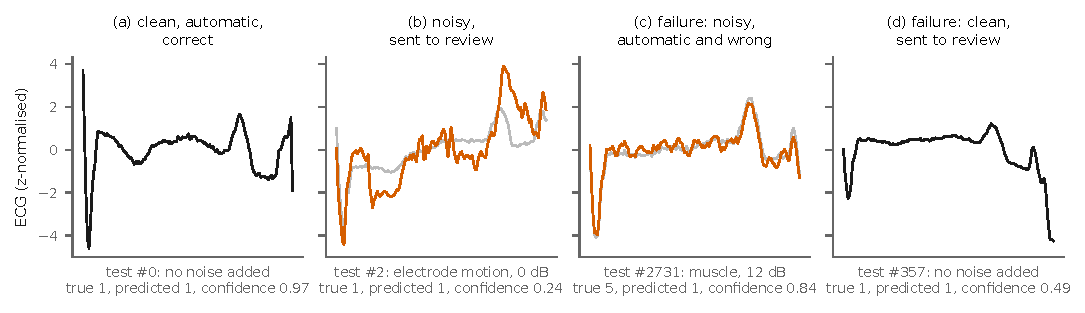
\includegraphics[width=\textwidth]{fig_qualitative.pdf}
\caption{LOOM flags most noisy recordings but misses some and sends some clean ones to review. Real-noise stream of ECG5000 (official split, LOOM, 20\,\% review budget). Rule: for each outcome, the first test recording in file order with that outcome. Grey: clean recording; orange: with NSTDB noise.}\label{fig:qualitative}
\end{figure*}

\subsection{Generality, sensitivity and sanity checks}\label{sec:general}
With MultiRocket features, LOOM compared with PreVal is \CmpMRFaults{} under faults and \CmpMRClean{} on clean data; with Hydra features it is \CmpHydraFaults{} under faults and \CmpHydraClean{} on clean data. On the \NUnseen{} datasets never used during development LOOM is \CmpUnseenFaults{} under faults; without datasets with exact duplicates \CmpNoDupFaults; without exact or near duplicates (\NNoNearDup{} datasets) \CmpNoNearDupFaults; and after merging datasets from the same source (\NGrouped{} units) \CmpGroupedFaults. With 25\,\% and 50\,\% of the training data, LOOM's median NLL under severity-3 faults is \TSTwentyFiveLoom{} and \TSFiftyLoom, against \TSTwentyFivePreVal{} and \TSFiftyPreVal{} for PreVal (\TSN{} datasets); \TSClaim. Under a real change of sensor (training on one accelerometer axis of UWaveGestureLibrary and testing on another), accuracy drops from \NSAccIn{} to \NSAccShift{} but leverage barely moves (median ratio \NSLevLo--\NSLevHi), and LOOM's advantage is small (mean NLL \NSNLLLoom{} vs \NSNLLPreVal, lower on \NSWins{} of \NSTasks{} axis pairs).

\label{sec:sanity}\emph{Sanity checks.} (1) Assumption~\ref{as:lev}: held-out and clean test leverages have the same median scale, but a Kolmogorov--Smirnov test rejects equal distributions on \ExchReject{} of \ExchN{} datasets (Holm-adjusted), so the assumption holds only approximately. (2) The spread of per-dataset jackknife+ coverage (standard deviation \CovSDObs) is larger than binomial sampling alone would give (\CovSDSim, 97.5\,\% quantile \CovSDSimHi); \CovOutside{} of datasets lie outside the binomial 95\,\% range, so coverage holds on average but not for every dataset. (3) Differences between LOOM and PreVal exceed two resampling standard errors on \NoiseCleanBeyond{} of the datasets on clean data and on \NoiseFaultsBeyond{} under faults, in favour of LOOM on \NoiseFaultsLoom{} of the datasets.

\subsection{Computational complexity and cost}\label{sec:cost}
LOOM costs the same to fit as PreVal (median \FitLoom\,s vs \FitPreVal\,s on top of the shared MiniRocket transform of \FitTransform\,s; Supplementary Table~\ref{S-tab:cost}). From raw data to a fitted model, LOOM takes about \FitEndToEndLoom\,s, against \FitQuant\,s for QUANT, \FitLoomEns\,s for a five-seed ensemble and \FitArsenal\,s for the Arsenal.

\subsection{Software tool}\label{sec:tool}
We release LOOM as a Python package with a command-line tool, \texttt{loom-triage}: \texttt{fit} trains a model on a CSV of labelled recordings, \texttt{run} writes a review queue with prediction, confidence, unusualness ($h/h_{\mathrm{ref}}$), decision and optional prediction set, plus an HTML report, and \texttt{evaluate} scores labelled data. The tool has its own unit tests and was validated end to end on plain CSV files outside the experimental pipeline (Supplementary Sect.~\ref{S-sec:tool}).

\subsection{Discussions}\label{sec:discussion}
LOOM uses a second quantity that the LOO algebra provides for free, the held-out leverage, to put each prediction on the scale of its own uncertainty. For an operator, this means that a LOOM model that is unsure about a recording is more likely to be looking at a damaged one, and that a fixed review budget catches about \CCaughtLoom{} rather than \CCaughtPreVal{} of the damaged recordings in our confirmatory study. QUANT classifies damaged recordings more accurately; it made the fewest automatic errors in the exploratory study and with real ECG noise, while in the confirmatory study LOOM's median automatic error was lower but not significantly. A tree ensemble for the label combined with LOOM's leverage for the review decision is a promising design. We would use LOOM when training sets are small, recordings may be damaged, and a single fast model is preferred; where test data are known to be clean, PreVal gives a lower clean calibration error.

The main limitations are:
\begin{enumerate}
\item Apart from the real ECG noise, all faults are simulated, and real noise was tested on ECG only; the noise was added at its native 360\,Hz sampling because the UCR files do not record their sampling rates. The only real change of sensor we studied barely moves leverage, and LOOM gains little there.
\item Leverage does not respond to changes that keep the features within the training range (speed variation, another sensor axis, label noise, changing class frequencies).
\item On clean data LOOM is not better than PreVal, and target smoothing raises its calibration error on datasets with few training series per class.
\item QUANT has a lower likelihood loss than LOOM under the strongest faults.
\item The jackknife+ guarantee holds only approximately (Assumption~\ref{as:fixed}), and per-dataset coverage varies more than sampling noise allows.
\item For compute reasons, ensembles, other extractors and the Arsenal were evaluated on the official split only, logistic regression was skipped for four large datasets, and deep networks were not run.
\item The exploratory triage study and several analyses were designed after the main results were known; they are labelled as post hoc (Supplementary Sect.~\ref{S-sec:deviations}).
\end{enumerate}

%=====================================================================
\section{Conclusion and future scope}\label{sec:conclusion}
We showed that a closed-form change to the readout of fast random-kernel classifiers makes their confidence drop for recordings far from the training data, without held-out data, refitting or ensembles. LOOM lowered the likelihood loss under simulated faults and real ECG noise compared with the strongest previous readout, and in a pre-registered triage study its review queue caught \CCaughtLoom{} instead of \CCaughtPreVal{} of the faulty recordings. We did not show an advantage on clean data or over the tree-based QUANT classifier under the strongest faults, and leverage does not detect changes that keep the features in range. Next steps are a study with expert-labelled real faulty recordings, multivariate signals, combining QUANT's trees with LOOM's leverage, and adaptive target smoothing for problems with many classes and few examples.

\backmatter

\bmhead{Supplementary information}
Supplementary Material: proofs, deviations log, leakage audit, fault definitions, software validation and additional tables and figures.

\bmhead{Acknowledgements}
An AI assistant (Claude, Anthropic) was used for the literature search, code, experiments and drafting, as described in Sect.~\ref{sec:framework}. [Further acknowledgements to be completed by the authors.]

\section*{Declarations}
\begin{itemize}
\item Funding: [to be completed by the authors]
\item Competing interests: [to be completed by the authors]
\item Ethics approval and consent to participate: not applicable (public, de-identified benchmark data).
\item Data availability: UCR archive (\url{https://www.timeseriesclassification.com}; free for research use with citation of \citet{dau2019ucr}) and MIT-BIH Noise Stress Test Database (\url{https://physionet.org/content/nstdb/1.0.0/}; Open Data Commons Attribution License v1.0).
\item Code availability: [public repository link to be inserted by the authors]; all results, tables, figures and the number macros of this paper are regenerated by one script.
\item Author contribution: [to be completed by the authors]
\end{itemize}

\bibliography{references}

\end{document}
